%%%%%%%%%%%%%%%%%%%%%%%%% %
% CH3 : Inviscid incompressible potential flows %
%%%%%%%%%%%%%%%%%%%%%%%%% %

\chapter{Inviscid incompressible potential flows}

\section{Introduction}
	\subsection{Governing equations}
		Let's remind that we have a set of 4 equations and 4 unknowns. It's inviscid so there are no stresses. These equations are decoupled from the energy equation, for constant density flows, the hydrodynamic problem gets decoupled from the thermal problem. So when we speak about compressible fluid we have to couple them. 
		\begin{equation}
			\rho = cst \qquad\qquad \nabla \vec{u} = 0 \qquad\qquad \rho \left[\frac{\D \vec{u}}{\D t} + \vec{u} \nabla \vec{u} \right] = -\nabla p +\rho \vec{F}
			\label{eq:3.1}
		\end{equation}
		
	\subsection{Bernouilli equation}
		The flow is barotropic, in additoin let's consider that the flow is steady and that the force derives from a potential $\vec{F} = -\nabla \Phi$ (F = 0 for most applications). We have the Bernouilli equation
		\begin{equation}
			\epsilon _m = \frac{p}{\rho}+k + \cancel{\Phi} = cst = \frac{p}{\rho} +\frac{u^2}{2}
		\end{equation}
		The mechanical energy is constant on a streamline. We can give an interpretation to the constant by writing it as $\frac{p_t}{\rho} = \frac{p^0}{\rho}$. Physically, $p^0$ is the pressure where u = 0 and is called \textbf{stagnation pressure}. The constant differs from streamline to streamline. Indeed we found that $\vec{\omega}\times \vec{u} = -\nabla \epsilon _m$, so if the fluid is rotational $\epsilon _m$ will differ from streamline to another, meaning that the stagnation pressure differs. 
		
	\subsection{Irrotational (potential) flow}
		In that case we have that $\omega = 0$ so $\vec{u} = \nabla \varphi$  ($\varphi$ beeing a velocity potential) and $p^0$ is the same for all streamlines : $\nabla p^0 = 0$. For incompressible flows, we have the definition 
		\begin{equation}
			p^0 = p+\frac{\rho u^2}{2}
		\end{equation}
		where the two terms are respectively the \textbf{static pressure} and the \textbf{dynamic pressure}. The definition $\vec{u}=\nabla \varphi$ can be introduced in \eqref{eq:3.1} to have 
		\begin{equation}
			\nabla \vec{u} = \nabla \nabla \varphi = \nabla ^2 \varphi
		\end{equation}
		which is \textbf{Laplace's equation}. His linearity makes it more solvable than Navier-Stokes equations and we are unable to get $\varphi \rightarrow \vec{u} \rightarrow p$ and we can use \textbf{superposition principle}. So if $\varphi _1$ and $\varphi _2$ are two solutions, then any linear combination $a\varphi _1 + b\varphi _2$ is also a solution. 
		
\section{Elementary planar (2D) flows}
	\subsection{Complex potential}
		We start from the previous general equation
		\begin{equation}
			\vec{u} = \nabla \varphi \qquad \Rightarrow \qquad
			\left\{
			\begin{aligned}
			u_1 &= \frac{\D \varphi}{\D x_1} = \frac{\D \psi}{\D x_2}\\
			u_2 &= \frac{\D \varphi}{\D x_2} = -\frac{\D \psi}{\D x_1}
			\end{aligned}
			\right.
			\label{eq:3.5}
		\end{equation}
		where the second equality comes from the streamfuntion \eqref{eq:1.111}. This is called the \textbf{Cauchy-Riemann equations} that a complex analytic function has to satisfy. So $\varphi + i \psi\equiv \chi (x_1 + ix_2)=\chi (z)$ is one of  that and we call it the \textbf{complex potential}. For $\psi$ we have \eqref{eq:1.113} which says, in case of irrotational flows 
		\begin{equation}
			\nabla \psi = - \omega = 0. 
		\end{equation}
		As $\chi$ is analytic, we can compute its derivative 
		\begin{equation}
			\frac{\D \chi}{\D x_1} = \frac{\D \chi}{\D z} \underbrace{\frac{\D z}{\D x_1}}_{=1} \qquad \Rightarrow \qquad \frac{\D \chi}{\D z} = \frac{\D}{\D x_1} (\varphi + i \psi) = \frac{\D \varphi}{\D x_1}+i\frac{\D \psi}{\D x_1} = u_1 - i u_2 \equiv w,
		\end{equation}
		where $w$ is the \textbf{complex velocity}. Let's compute the integral over some curl of w 
		\begin{equation}
			\int _C w\, dz= \int _C (u_1 - i u_2)\, (dx_1 + idx_2) = \int _C \underbrace{u_1\, dx_1 + u_2\, dx_2}_{\vec{u}\, d\vec{s}} + i \int _C u_1\, dx_2 - u_2\, dx_1
		\end{equation}
		where $\vec{u}\, d\vec{s}$ is the work of the velocity. This beeing true for all curls, it's in particular true for a closed curl 
		\begin{equation}
			\oint w\, dz = \underbrace{\oint \vec{u}\, d\vec{s}}_{\Gamma} + i \underbrace{\oint u_1\, dx_2 - u_1\, dx_2}_{\dot{V}}
			\label{eq:3.9}
		\end{equation}
		where $\Gamma$ is the \textbf{circulation}. For the second term, let's remind the discussion in \eqref{eq:1.109} where we found $\vec{n} = \frac{dx_2}{ds}\vec{e}_1-\frac{dx_1}{ds}\vec{e}_2 \Rightarrow \vec{u}\vec{n}\, ds = u_1\, dx_2 -u_2\, dx_1$. This is exactly the second term integrated in \eqref{eq:3.9} where $\dot{V}$ corresponds to the \textbf{volume flow out of the closed contour}. A property of analytic functions is that its derivative is analytic and if it's analytic \textbf{everywhere inside the contour}, 
		\begin{equation}
			\oint _C w\, dz = \Gamma +i\dot{V} \neq 0
		\end{equation}
		\textbf{only if there are singularities inside the contour}. 
		
	\subsection{Uniform flow}
		This is the first elementary flow we will study is the case of a uniform flow along $x_1$ axis 
		\begin{equation}
		\left. \begin{aligned}
		u_1 &= u_\infty\\
		u_2 &= 0
		\end{aligned}
		\right\} 
		 \rightarrow w = u_\infty  \qquad \Rightarrow \qquad \chi = u_\infty z \rightarrow 
		 \left\{
		 \begin{aligned}
		 \varphi &= u_\infty x_1\\
		 \psi &= u_\infty x_2
		 \end{aligned}
		 \right.
		 .
		\end{equation}		 
		\begin{wrapfigure}[7]{l}{3.5cm}
		\vspace{-5mm}
		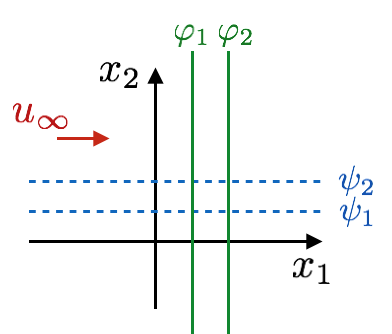
\includegraphics[scale=0.48]{ch3/1}
		\captionof{figure}{}
		\label{fig:3.1}
		\end{wrapfigure}		
		This means that streamlines are lines with constant $x_2$ and equi-potential lines with constant $x_1$ as represented on \autoref{fig:3.1}. In fact, if we remind \eqref{eq:3.5} the scalar 
		\begin{equation}
			\nabla \varphi \cdot \nabla \psi = \frac{\D \varphi}{\D x_1}\frac{\D \psi}{\D x_1} + \frac{\D \varphi}{\D x_2}\frac{\D \psi}{\D x_1} = -u_1u_2 +u_2u_1 = 0.
		\end{equation}
		\ \\ This means that the equi-potential lines and streamlines must be perpendicular. If we have a uniform flow with an angle $\alpha$ with respect to $x_1$, then 
		\begin{equation}
		\begin{array}{c}
			\left. \begin{aligned}
		u_1 &= u_\infty\cos \alpha\\
		u_2 &= u_\infty \sin \alpha
		\end{aligned}
		\right\} 
		 \rightarrow w = u_\infty(\cos \alpha - i\sin \alpha ) = u_\infty e^{-i\alpha} \\
		 \qquad \Downarrow \qquad \\
		 \chi = u_\infty ze^{-i\alpha} \rightarrow 
		 \left\{
		 \begin{aligned}
		 \varphi &= \operatorname{Re}(\chi ) = u_\infty (x_1\cos \alpha + x_2\sin \alpha )\\
		 \psi &= \operatorname{Im}(\chi ) = u_\infty (x_2\cos \alpha - x_1 \sin \alpha) \Leftrightarrow x_2 = x_1 \tan \alpha + \frac{\psi}{u_\infty}
		 \end{aligned}
		 \right.
		\end{array}
		\end{equation}
		where we see that the equation for $\psi$ is a line with angle $\alpha$. 
		
	\subsection{Source flow}
		\begin{wrapfigure}[5]{r}{5cm}
		\vspace{-5mm}
		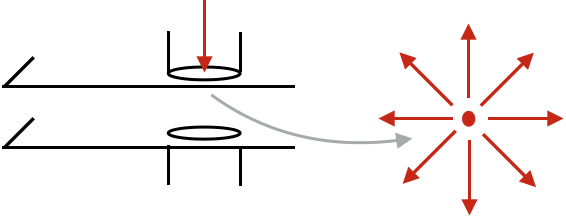
\includegraphics[scale=0.5]{ch3/2}
		\captionof{figure}{}
		\label{fig:3.2}
		\end{wrapfigure}		
		Let's imagine two plates separated by a fluid and a pipe on both surfaces allowing to inject fluid at some point. In reality fluid has a certain dimension but let's imagine that we word in 0 dimension. The point of impact can be represented as in red on \autoref{fig:3.2} and the symetry considerations can be made : 
		\ \\
		\begin{itemize}
			\item[•] The flow is radial : $\vec{u} = u_r \vec{e}_r$
			\item[•] Azimuthal symetry : $\frac{\D u_r}{\D \theta} = 0\qquad \Rightarrow u_r = f(r)$\\
		\end{itemize}
		If we define $\theta$ the angle with respect to horizontal axis, we have 
		\begin{equation}
			\vec{u} = f(r) \vec{e}_r = f(r) (\cos \theta \vec{e}_1 + \sin \theta \vec{e}_2)  \Rightarrow \left\{
			\begin{aligned}
			u_1 = f(r) \cos \theta \\
			u_2 = f(r) \sin \theta
			\end{aligned}
			\right.
			\qquad
			\Rightarrow 
			w = f(r)e^{-i\theta}.
		\end{equation}
		If we consider a closed curl of radius $r$ around the source, there is no circulation because streamlines are perpendicular. Considering polar coordinates, $z = re^{i\theta}$ and $dz = ire^{i\theta}\, d\theta$ 
		\begin{equation}
			\oint _C wdz = i\dot{V} = \int _0^{2\pi} f(r) e^{-i\theta}   ire^{i\theta}\, d\theta = ir f(r) 2\pi.
		\end{equation}
		There is a volume flux going out of the source and the function $f(r)$ is given by (with $\log z = \ln r + i\theta$)
		\begin{equation}
		\begin{aligned}
			f(r) = \frac{\dot{V}}{2\pi r} \qquad \Rightarrow w = \frac{\dot{V}}{2\pi r}e^{-i\theta} = \frac{\dot{V}}{2\pi z} \qquad \Rightarrow \chi = \frac{\dot{V}}{2\pi}\log z\\
			\Rightarrow \qquad \varphi = \operatorname{Re}(\chi ) = \frac{\dot{V}}{2\pi}\ln r \qquad and \qquad \psi = \operatorname{Im}(\chi ) = \frac{\dot{V}}{2\pi} \theta
		\end{aligned}
		\end{equation}		 
		\newpage
		\begin{wrapfigure}[8]{l}{3.5cm}
		\vspace{-1mm}
		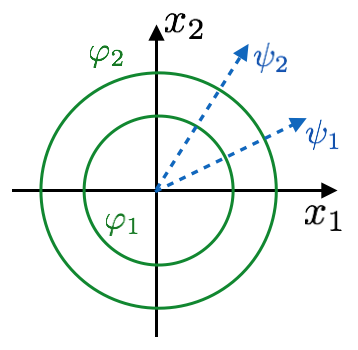
\includegraphics[scale=0.5]{ch3/3}
		\captionof{figure}{}
		\label{fig:3.3}
		\end{wrapfigure}
		We see that streamlines are lines with constant $\theta$ and equi-potential lines are circles of constant radius $r$ centered at the origin (\autoref{fig:3.3}). Notice that they are perpendiculat as the previous case. The source flow corresponds to \textbf{Green function} for fluids. Let's finally consider the case where the source is not located at the center but at a point $z_0$. We only have to make a shift of coordinates 
		\begin{equation}
			\chi = \frac{\dot{V}}{2\pi}\log (z-z_0).
		\end{equation}
		
	\subsection{Concentrated vortex flow}
		We will make an analogy with electricity. We know that vorticity and the current density are defined as
		\begin{equation}
			\vec{\omega} = \nabla \times \vec{u} \qquad \vec{J} = \nabla \times \vec{H}
		\end{equation}
		where $\vec{H}$ is the magnetic field. $\vec{J}$ is nothing else but the current in amperes divided by the surface of the electrical wire within the current circulates. With application of Stoke's theorem, we have
		\begin{equation}
			I = \int _S \vec{J}\vec{n}\, dS = \oint _C \vec{H}\, d\vec{S}.
		\end{equation} 
		We can, similarly to the current tube, define a vortex tube with 
		\begin{equation}
			\int _S \vec{\omega} \vec{n}\, dS = \oint _C \vec{u}\, d\vec{S} = \Gamma 
		\end{equation}
		\begin{wrapfigure}[8]{r}{3.5cm}
		\vspace{-5mm}
		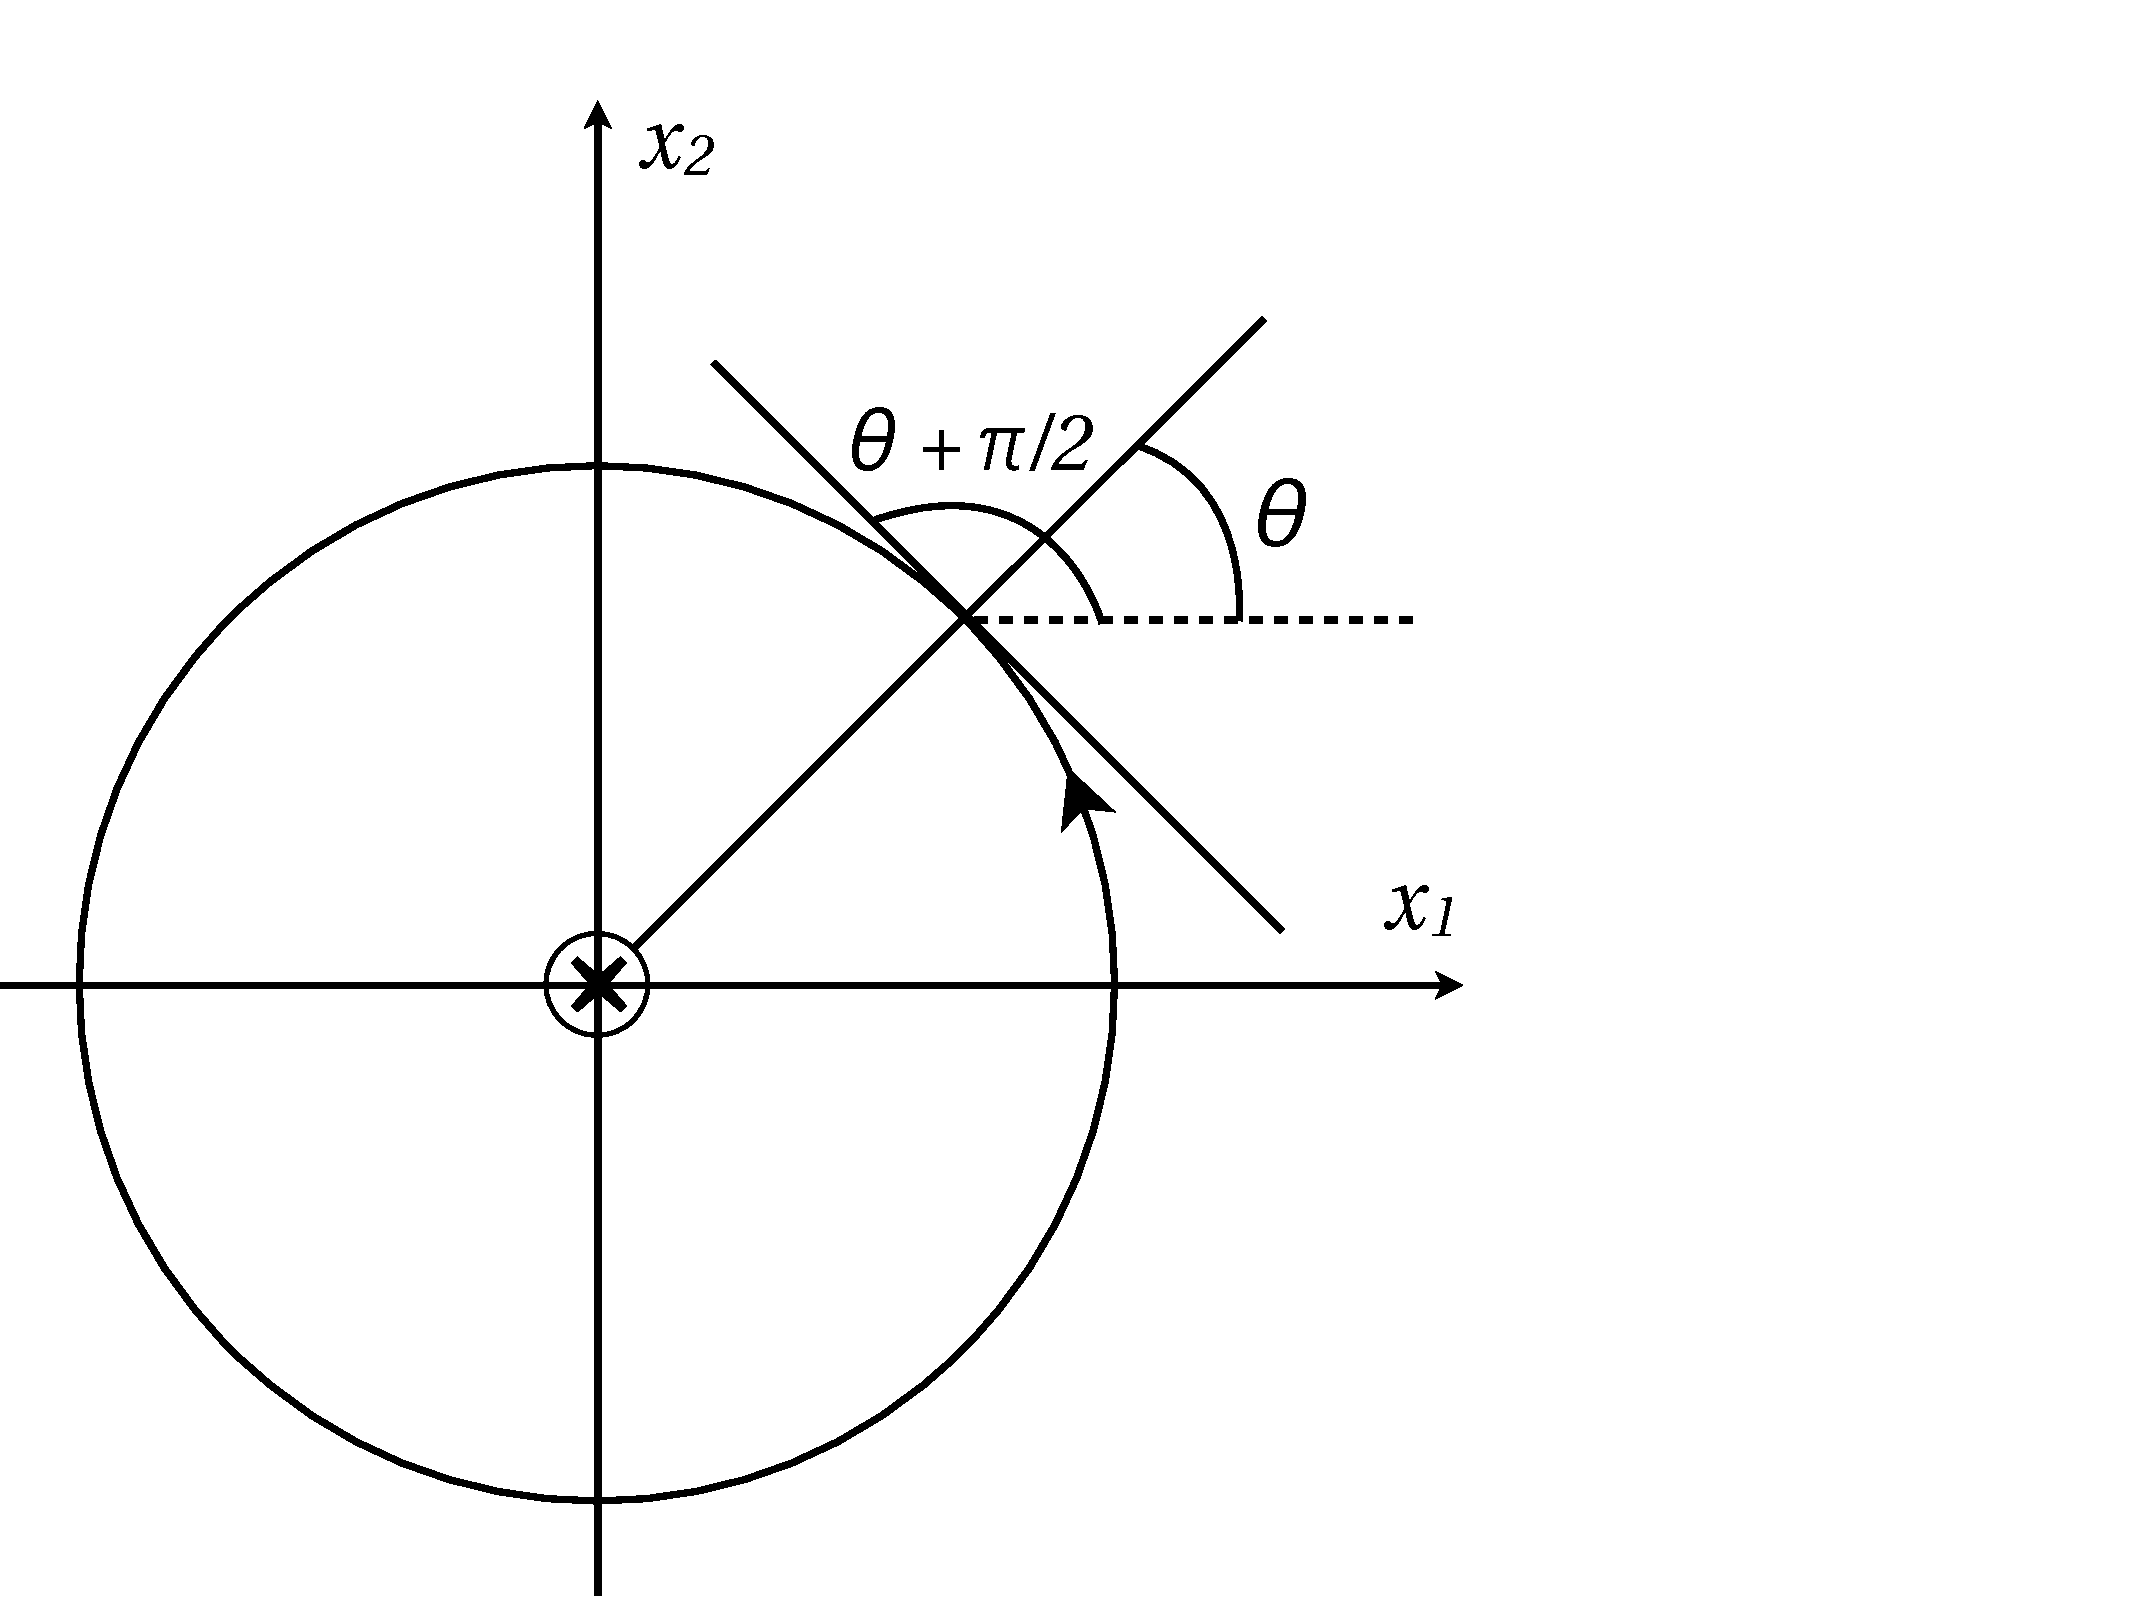
\includegraphics[scale=0.14]{ch3/5}
		\captionof{figure}{}
		\end{wrapfigure}
		where we find the \textbf{circulation} $\Gamma$. Actually when we model a wire, we do not consider a 2D section but concentrate the current over a line. We make the same with $\Gamma$ and look for the velocity field associated to the concentrated vortex tube (same as looking for $\vec{H}$ associated to concentrated $I$). For a concentrated current, we have an azimuthal magnetic field with an azimuthal symetry (circles), so this is the same for $\vec{u}$
		\begin{equation}
			\vec{H} = H_\theta \vec{e}_\theta \qquad \Rightarrow \vec{u} = \underbrace{u_\theta (r)}_{f(r)} \vec{e}_\theta
		\end{equation}
		where $f(r)$ will be determine as in the previous section but $\theta$ becomes $\theta +\pi /2$ due to $\vec{e}_r \perp \vec{e}_\theta$
		\begin{equation}
		\left.
			\begin{aligned}
			u_1 &= f(r) \cos (\theta +\pi /2) = -f(r)\sin \theta \\
			u_2 &= f(r) \sin (\theta +\pi /2) = f(r) \cos \theta
			\end{aligned}
			\right\}
			\quad \Rightarrow 
			\begin{aligned}
			w = u_1 - iu_2 = f(r) (i^2 \sin \theta - i \cos \theta)\\
				= -i f(r) (\cos \theta - i \sin \theta )= -i f(r) e^{-i\theta}
			\end{aligned}
		\end{equation}
		And if we integrate over a closed curl and equalize to $\Gamma$ ($\dot{V}=0$) 
		\begin{equation}
			\oint _C w\, dz = -i\, ir f(r)2\pi = \Gamma \qquad \Rightarrow \qquad f(r) = \frac{\gamma}{2\pi r}.
		\end{equation}
		And so 
		\begin{equation}
			w = -i \frac{\Gamma}{2\pi r}e^{-i\theta} = -i \frac{\Gamma}{2\pi z} \qquad \Rightarrow \chi = -\frac{\Gamma}{2\pi}\log z \qquad \Rightarrow \varphi = \frac{\Gamma}{2\pi} \theta \qquad \psi = -\frac{\Gamma}{2\pi}\ln r
		\end{equation}
		As conclusion, we see that streamlines are lines of constant $r$ (circles) and equi-potential lines lines of constant $\theta$. It is the same as \autoref{fig:3.3} except that we have an exchange between $\varphi$ and $\psi$. This exchange is due to the $-i$ factor. 
		
		\newpage
		
	\subsection{Fluid dipole - doublet}
		\begin{wrapfigure}[6]{l}{6.5cm}
		\vspace{0mm}	
		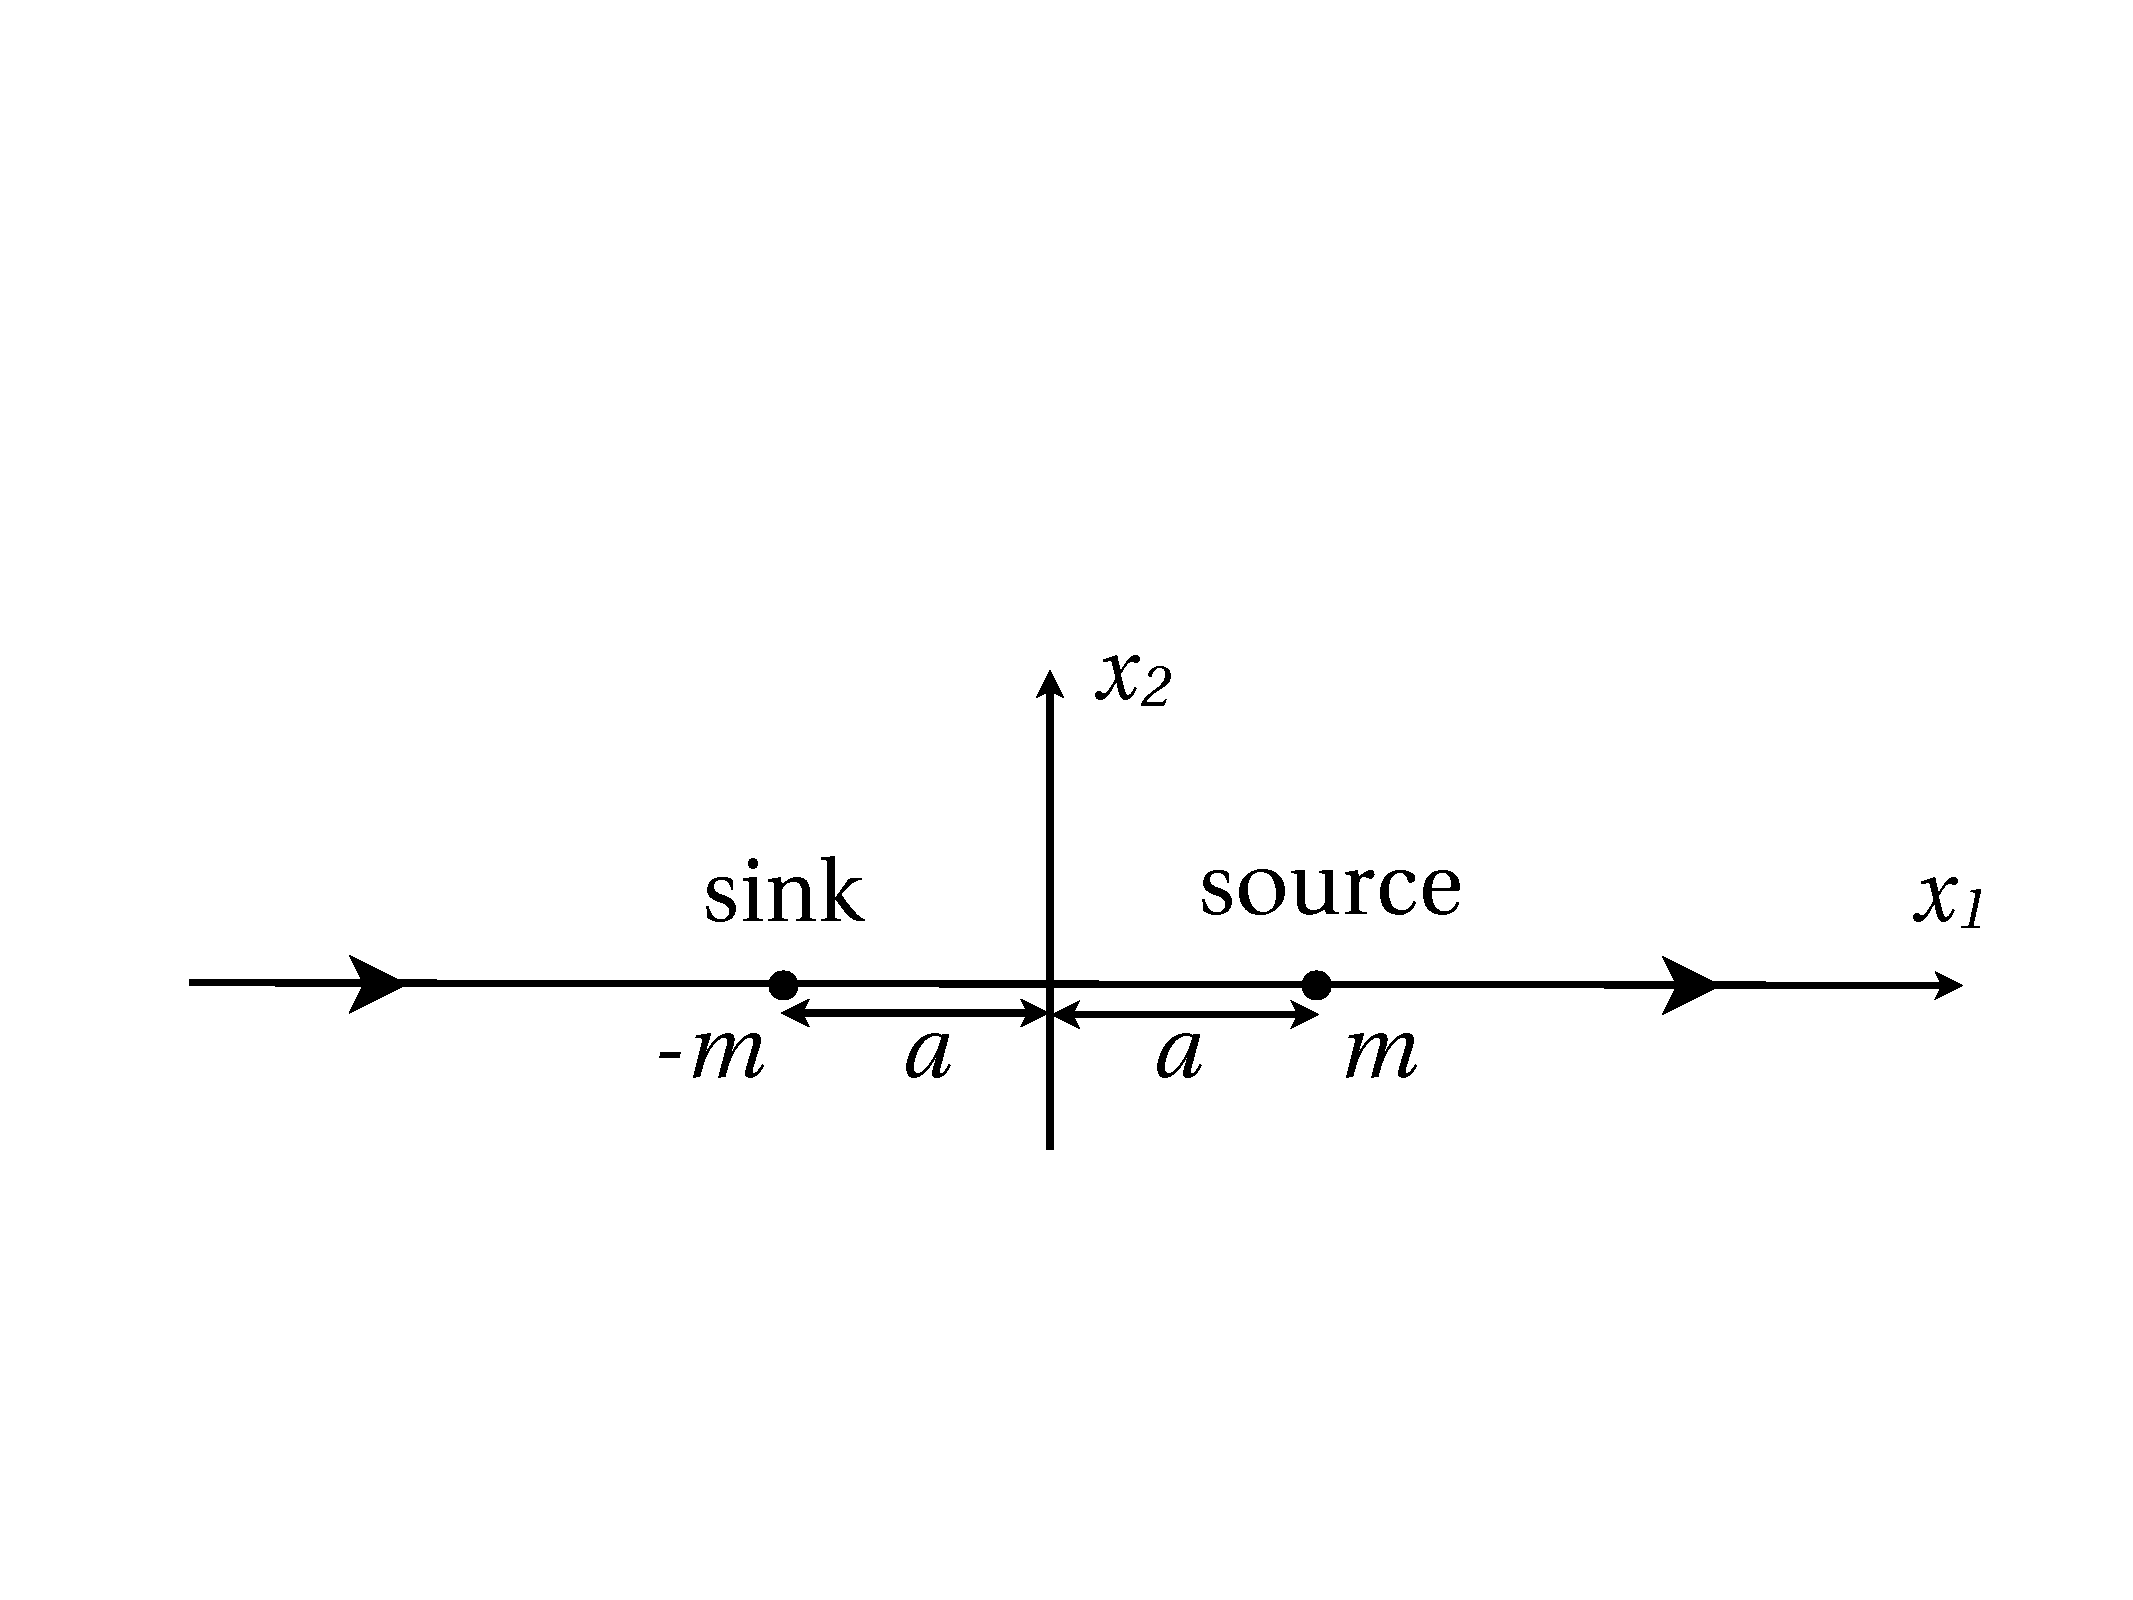
\includegraphics[scale=0.2]{ch3/4}	
		\captionof{figure}{}
		\end{wrapfigure}
		The idea is to build more complex designs. If we have a source of volume flow $\dot{V}$ located on $+a$ and a source with $-\dot{V}$ (a sink) at $-a$. We let then $a\rightarrow 0$, but if $a=0$, the sources are superposed and there is no flow. To remediate, we let $\dot{V}\rightarrow \infty$ as $a\rightarrow 0$, such that $\dot{V}\times 2a= \mu = cst$. For a finate a 
		\begin{equation}
		\begin{aligned}
			\chi = \chi _{source} + \chi _{sink} = \frac{-\dot{V}}{2\pi}&\log (z-a) + \frac{\dot{V}}{2\pi}\log (z+a) = \frac{\dot{V}}{2\pi} (\log (z-a) - (\log (z+a))\\
			 &= \frac{\dot{V}}{2\pi} \log \frac{z-a}{z+a} = \frac{\dot{V}}{2\pi} \log \left( 1+ \frac{2a}{z+a} \right)
		\end{aligned}
		\label{eq:3.25}
		\end{equation}
		Because of $a\rightarrow 0$, we can make an expansion knowing that $\frac{1}{1-t}$ is the sum of a geometric series 
		\begin{equation}
			\ln (1-t) = \int \frac{1}{1-t} \, dt = - \left( \int (1+t+t^2+...) \, dt \right) = -t-\frac{t^2}{2}-\frac{t^3}{3}+... 
		\end{equation}
		Replacing this in \eqref{eq:3.25}
		\begin{equation}
			\chi = \frac{\dot{V}}{2\pi} \left(- \frac{2a}{z+a}- \frac{4a^2}{2(z+a)^2} + ... \right) = -\frac{\mu}{2\pi(z+a)}-\frac{\mu a}{(z+a)^2}+ ...
		\end{equation}

		\begin{wrapfigure}[8]{r}{3.2cm}
		\vspace{-5mm}	
		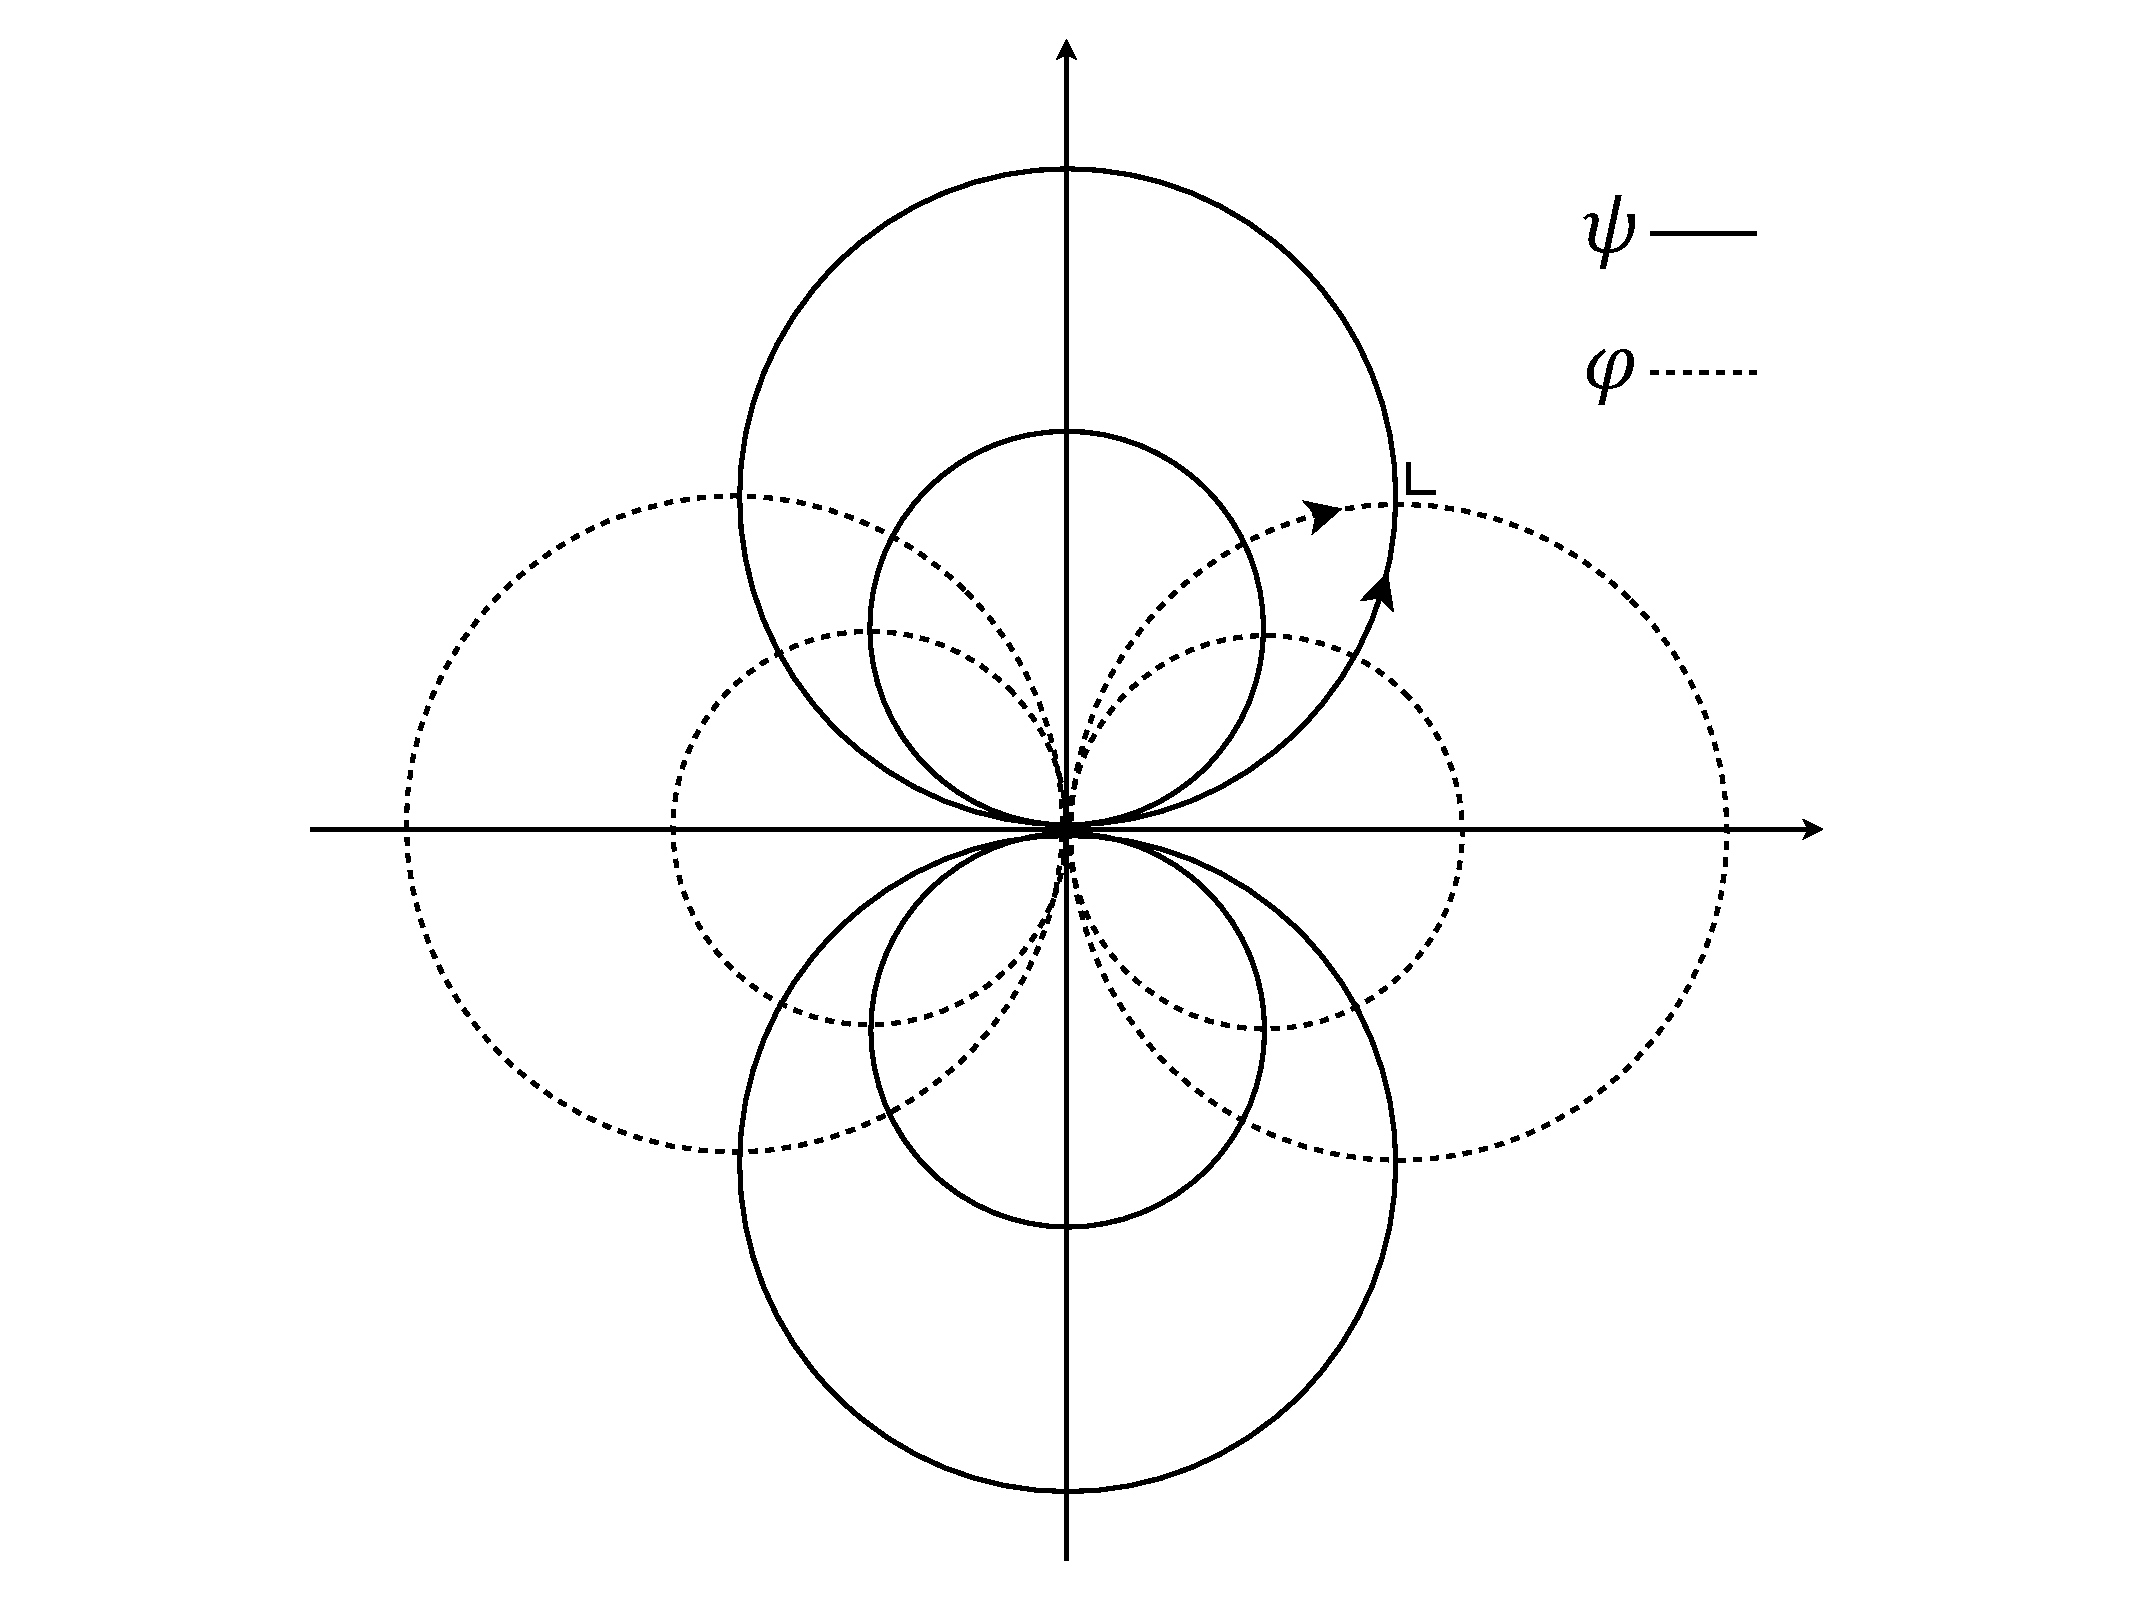
\includegraphics[scale=0.12]{ch3/6}	
		\captionof{figure}{}
		\label{fig:3.6}
		\end{wrapfigure}
		In the limit $a\rightarrow 0$ 
		\begin{equation}
			\chi _{dipole} = -\frac{\mu}{2\pi z} \qquad and \qquad w= \frac{\mu}{2\pi z^2}.
		\end{equation}
		This makes sense because $w\geq 0$ means that the source pushes the fluid to the right and so the sink sucks the fluid from left to right. So when z is a real, $w$ should be positive. We see that a dipole has a certain direction to the contrary of the vortices and sources. Before computing $\psi$ and $\varphi$, let's remind that
		\begin{equation}
			\frac{1}{z} = \frac{x_1-ix_2}{x_1^2+x_2^2} \qquad \Rightarrow \psi = \operatorname{Im}(-\frac{\mu}{2\pi z}) = \frac{\mu}{2\pi}\frac{x_2}{x_1^2+x_2^2} \qquad \Leftrightarrow x_1^2+x_2^2-\frac{\mu}{2\pi\psi}x_2 = 0
		\end{equation}
		This last equation corresponds to a circle going throw the origin and since $x_2$ is in the linear part, the center is on $x_2$ axis. We do the same for $\varphi$ with taking 
		\begin{equation}
			\varphi = \operatorname{Re}(\chi) = -\frac{\mu}{2\pi}\frac{x_1}{x_1^2+x_2^2} \qquad \Leftrightarrow \qquad x_1^2+x_2^2+\frac{\mu}{2\pi\varphi}x_1 = 0.
		\end{equation}
		We see that $(0,0) \in \varphi$ too and now the center is on $x_1$ axis (\autoref{fig:3.6}). 
		

\section{Force and torque on a body in an incompressible plana (2D) potential flow}
	\begin{wrapfigure}[3]{l}{3.6cm}
		\vspace{-10mm}	
		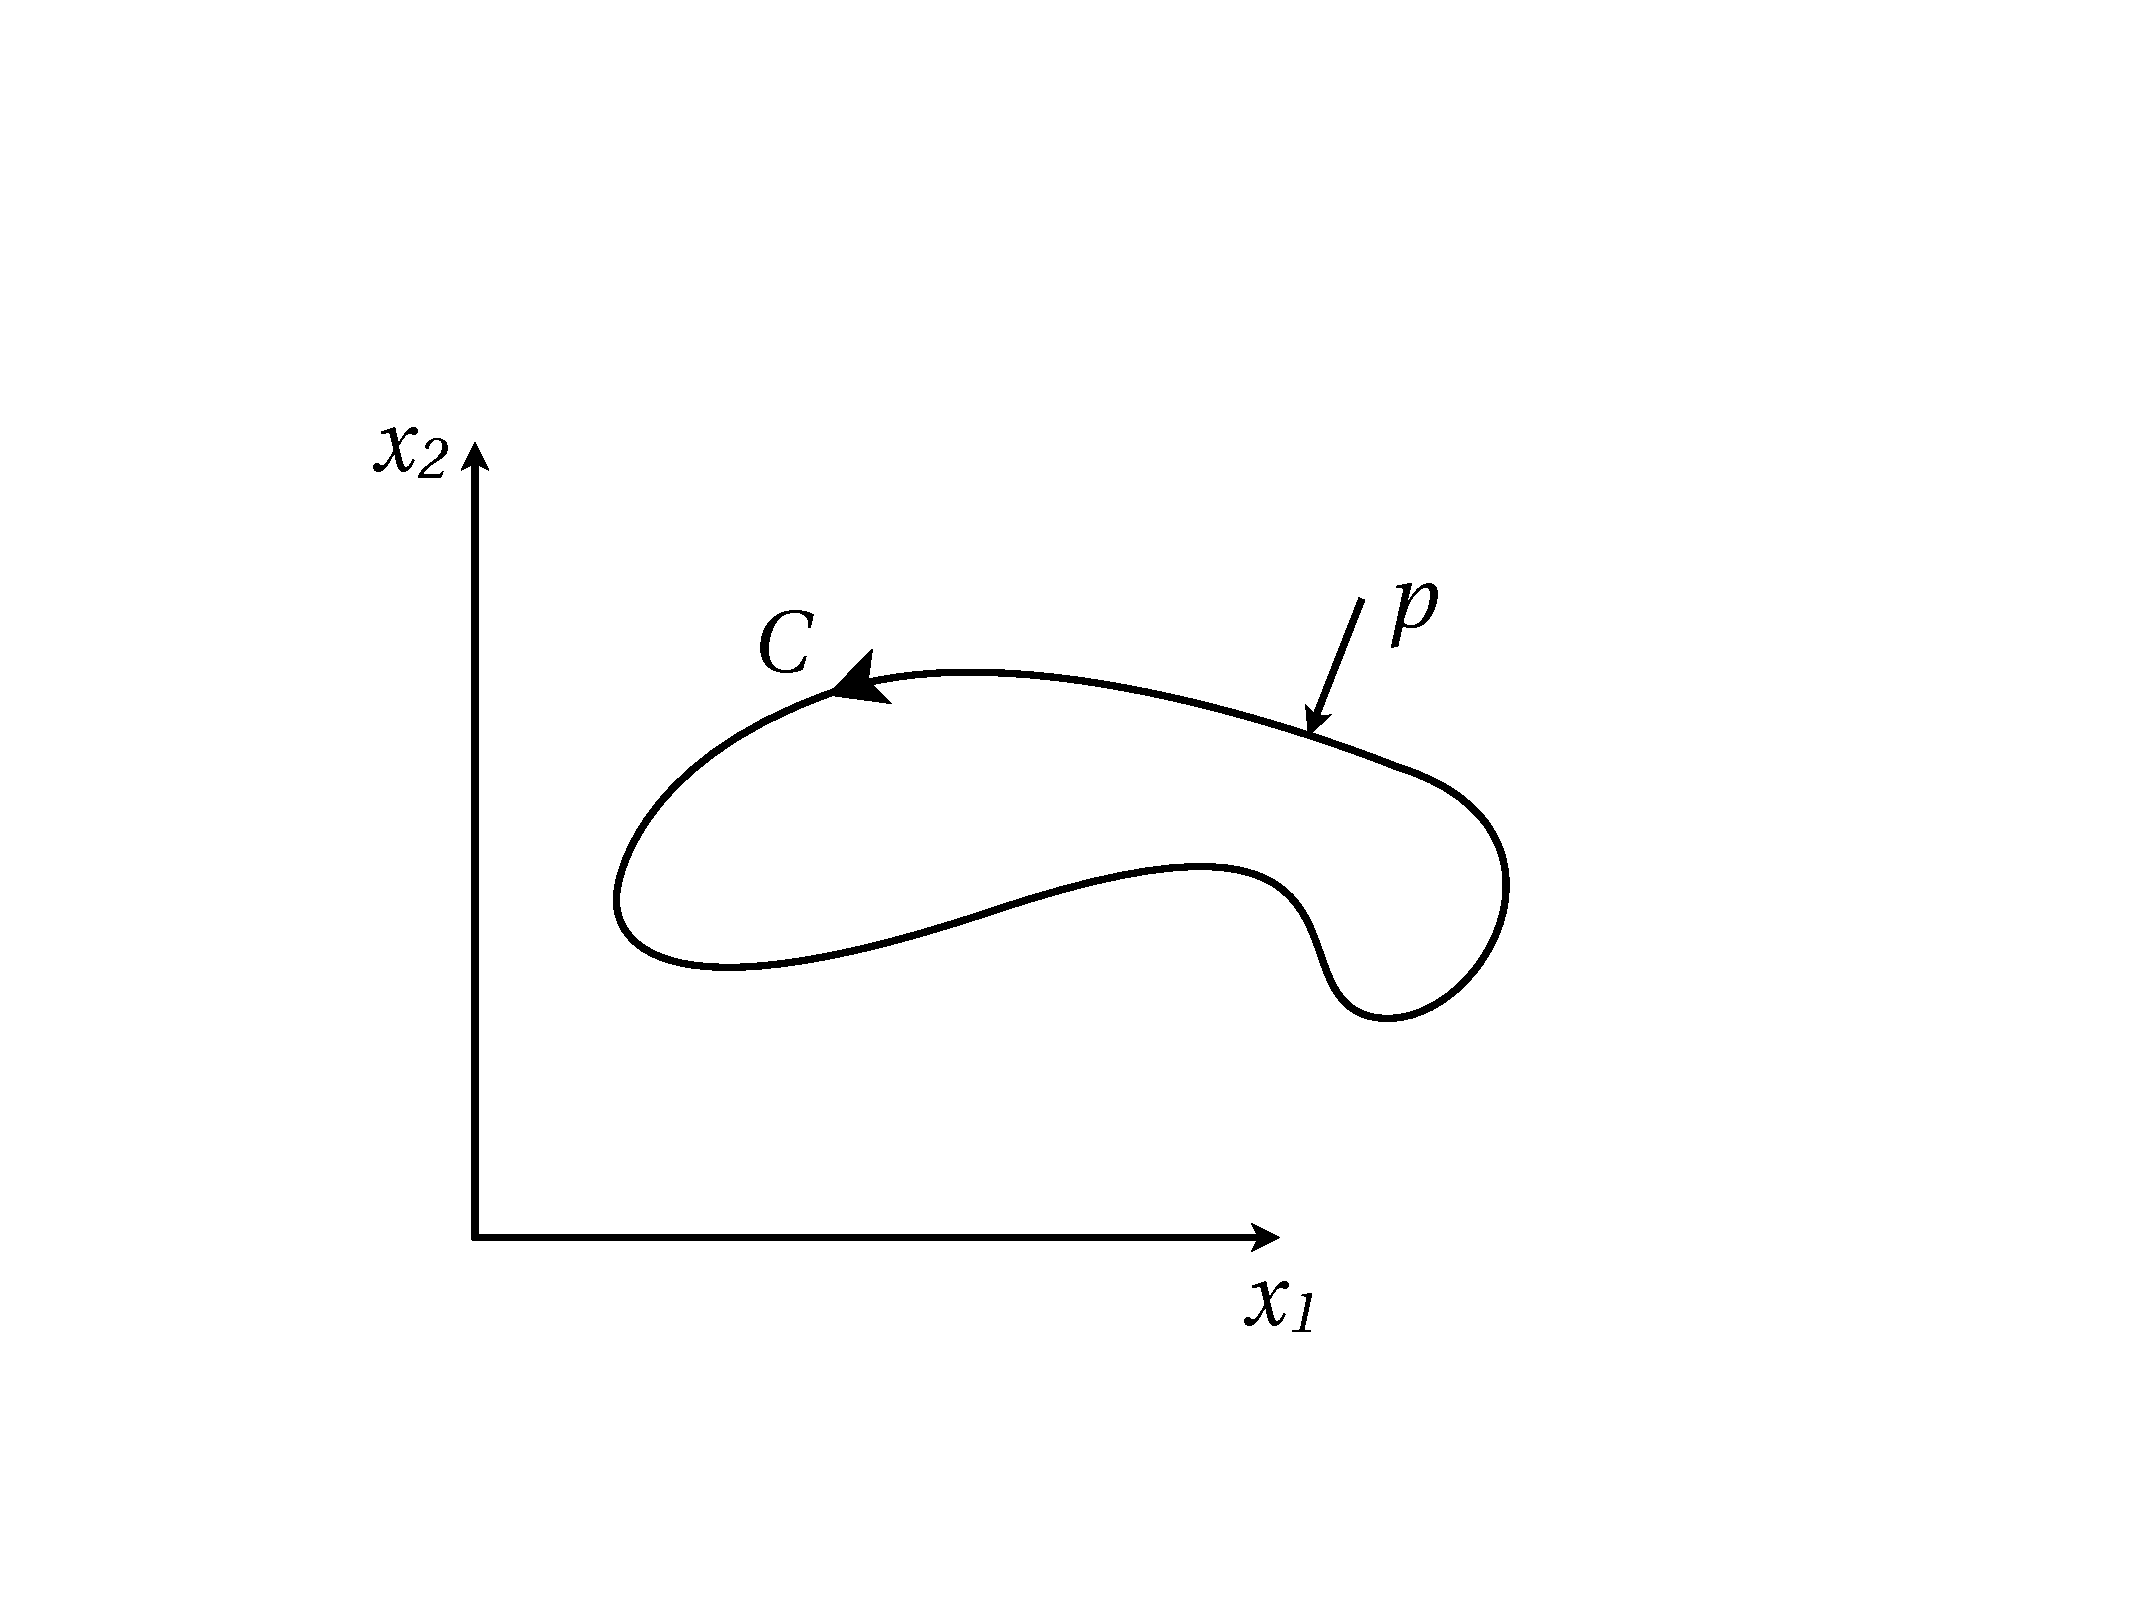
\includegraphics[scale=0.18]{ch3/7}	
		\captionof{figure}{}
		\end{wrapfigure}
		We will create more complex flows by assumbling these elementary solutions but we need a theorem useful to compute forces on a solid body in a potential flow. Let's consider the surface forces on a solid body. For \textbf{invicid flows}, the only component is the \textbf{pressure}. The elementary force given by $p\, ds (-\vec{n})$\footnote{s here is not a surface because we have 2D flows, we speak about "per unit span/length" (a distance normal to the plan of the flow).}, we have \footnote{$n_1\, ds = dx_2, n_2 \, ds = dx_1$ by \eqref{eq:1.109}}
	\begin{equation}
		\vec{F} = -\oint _C p\vec{n}\,ds \qquad with \qquad
		\left\{
		\begin{aligned}
		F_1 &= -\oint _C pn_1\,ds = - \oint p \, dx_2\\
		F_2 &= -\oint _C pn_2\,ds =  \oint p \, dx_1
		\end{aligned}
		\right.
	\end{equation}
	It's interesting to compute a complex number like previously 
	\begin{equation}
		F_1 - i F_2 = - \oint_C p (-i^2 dx_2 + i dx_1) = - i \oint_C p \underbrace{(dx_1 - i dx_2)}_{d\bar{z}}. 
	\end{equation}
	
	We know that the pressure is linked to the velocity by Bernoulli's theorem 
	\begin{equation}
	p + \rho \frac{u^2}{2} = p +\rho \frac{u_1^2+u_2^2}{2} = p +\rho \frac{w	\bar{w}}{2} = cst = p_t \qquad \Rightarrow p = p_t - \rho \frac{w	\bar{w}}{2}
	\end{equation}
	where $p_t$ is called the \textbf{total or stagnation pressure}. By replacing this in previous equation, we have
	
	\begin{equation}
		F_1 - i F_2 = -i \oint_C \left(p_t - \rho\frac{w \bar{w}}{2}\right) \, d\bar{z}.
	\end{equation}
	Let's check the contribution of each term. I say that contribution of $p_t$ is null, the proof :
	\begin{itemize}
		\item[•] Mathematical proof : \\
		Whe have the integral over a closed contour of an exact differantial, so $p_t\oint dx_1 = 0$.
		\item[•] Physical proof : \\
		If we have a pressure applied somewhere, it exists another pressure exactly opposed somewhere else that cancels this first one for a cst $p_t$. \\
	\end{itemize}
	
	Therefore 
	\begin{equation}
	F_1 - i F_2 = \frac{\rho}{2}i \oint_C  w \overline{w} \, d\bar{z}.
	\end{equation}
	The contour has to be taken on the solid and there we have the tangential conditions, the fluid has to flow tangentially to the body. Let's compute $w\, dz$
	\begin{equation}
	\begin{aligned}
	w \, dz &= (u_1 - i u_2) (dx_1 + i dx_2) \\
 				&= u_1 dx_1 + u_2 dx_2 + i \underbrace{(u_1 dx_2 - u_2 dx_1)}_{\vec{u}.	\vec{n} \, ds = 0 \mbox{ (no penetration)}}\\
				&= u_1 dx_1 + u_2 dx_2
	\end{aligned}
\end{equation}
	This beeing a pure real, it's equal to its conjugate $\bar{w}\, d\bar{z}$. We finally have the 
	
	\begin{center}
	\theor{\textbf{Blasius formula for forces}
	\begin{equation}
		F_1 - i F_2 = \frac{\rho i}{2} \oint_C  w^2  \, dz
	\end{equation}
	}
	\end{center}
	Now, what about the torque of the force? It's defined as 
	\begin{equation}
	d\vec{C} = \vec{x} \times (-p\vec{n} \, ds) = \left|
\begin{array}{ccc}
\vec{e}_1 & \vec{e}_2 & \vec{e}_3\\
x_1 & x_2 & 0\\
-pn_1 & -pn_2 & 0 \\
\end{array}
\right|
=dC_3 = \left( x_1 dx_1 + x_2 dx_2\right) p= \Re \left( pz \ d\overline{z} \right)
	\end{equation}
	By integrating this along a contour and recognizing $x_1dx_1+x_2dx_2 = \frac{d(x_1^2+x_2^2)}{2} = \frac{d(z\bar{z})}{2}=\frac{z\, d\bar{z}+\bar{z}\, dz}{2} = \operatorname{Re}(\bar{z}\, dz)$, we have 
	\begin{equation}
		C_3 = \oint p\operatorname{Re}(\bar{z}\, dz) = \oint (\cancel{p_t} - \rho \frac{w\bar{w}}{2})\operatorname{Re}(\bar{z}\, dz) = -\operatorname{Re}\left(\oint \rho \frac{w\bar{w}}{2}\bar{z}\, dz \right).
	\end{equation}
	Finally, $w\, dz = \bar{w}\, d\bar{z}$ for the same reason as $w\,dz$, giving the 
	
	\begin{center}
	\theor{\textbf{Blasius formula for torques}
	\begin{equation}
		C_3 = -\frac{\rho}{2}\operatorname{Re}\left(\oint w^2\bar{z}z\, dz \right)
	\end{equation}
	}
	\end{center}
	We will use that to get the expression of force over an arbitrary body immersed in an otherwise uniform flow, consider $u_\infty$ as describing an angle $\alpha$ with $x_1$ axis. e know from the previous sections that the $w(z)$ is a complex analytical function outside $C$ (inside there is no fluid $\rightarrow$ singularity). So $w(z)$ is analytical outside a circle centered at the origin and it can be explanded in Laurent series
	\begin{equation}
		w(z) = \sum_{n=0}^\infty a_n z^n + \sum_{m=1}^\infty\frac{b_m}{z^m}
	\end{equation}
	When we take account that the fluid has $u_\infty$ in the far field (uniform), we know that the second part will tend to zero, so the first part must be a cst
	\begin{equation}
		\lim _{z\rightarrow \infty} w(z) = u_\infty e^{-i\alpha} \equiv w_\infty \qquad \Rightarrow a_n = 0 \, (n>0) \quad and \quad a_0 = w_\infty .
	\end{equation}
	
	We also know that by the Laurent's theorem 
	\begin{equation}
	b_m = \frac{1}{2 \pi i} \oint w(z) z^{m-1} \ dz\qquad \Rightarrow \qquad
	b_1 = \frac{1}{2 \pi i} \oint w(z) \ dz = \frac{1}{2 \pi i} \left(\Gamma + i 	\cancel{\dot{V}}\right) = \frac{\Gamma}{2\pi i} 
	\end{equation}
	where $\dot{V}=0$ because there is no volume flow out, as the body is closed. 	Therefore,
	\begin{equation} 
	w(z) = w_\infty + \frac{\Gamma}{2 \pi i z} 
	+ \sum_{m=2}^\infty \frac{b_m}{z^m}.
	\end{equation} 
	This allows us to compute $w^2$ that matters for us, as the product of itself by itself
	
	\begin{equation}
	\begin{aligned}
	 w^2(z)&= \left( w_\infty + \frac{\Gamma}{2 \pi i z} 
	+ \frac{b_2}{z^2} + \cdots \right) \left( w_\infty + \frac{\Gamma}{2 \pi i z} 
	+ \frac{b_2}{z^2} + \cdots \right) \\
	&= w_\infty^2 + \frac{2 w_\infty \Gamma}{2 \pi i z} + \frac{1}{z^2}\left( -\frac{\Gamma ^2}{4\pi^2}+2b_2w_\infty\right) + \cdots \\
	&= A_0 + \frac{B_1}{z} + \frac{B_2}{z^2}+\cdots \qquad with \qquad B_1= \frac{2w_\infty \Gamma }{2 \pi i}
	\end{aligned}
	\end{equation}
	Now if we use Laurent theorem reversed, we find 
	\begin{equation}
		\oint _C w^2(z) \, dz = 2\pi i B_1 = 2w_\infty \Gamma .
	\end{equation}
	This applied to the Blasius force gives 
	\begin{equation}
	 F_1- iF_2 = \frac{\rho i}{2} 2w_\infty \Gamma = \rho i u_\infty e^{-i\alpha} \Gamma = \rho u_\infty \Gamma e^{-i(\alpha -\pi /2)}.
	\end{equation}

	\begin{wrapfigure}[8]{l}{3.6cm}
		\vspace{-0mm}	
		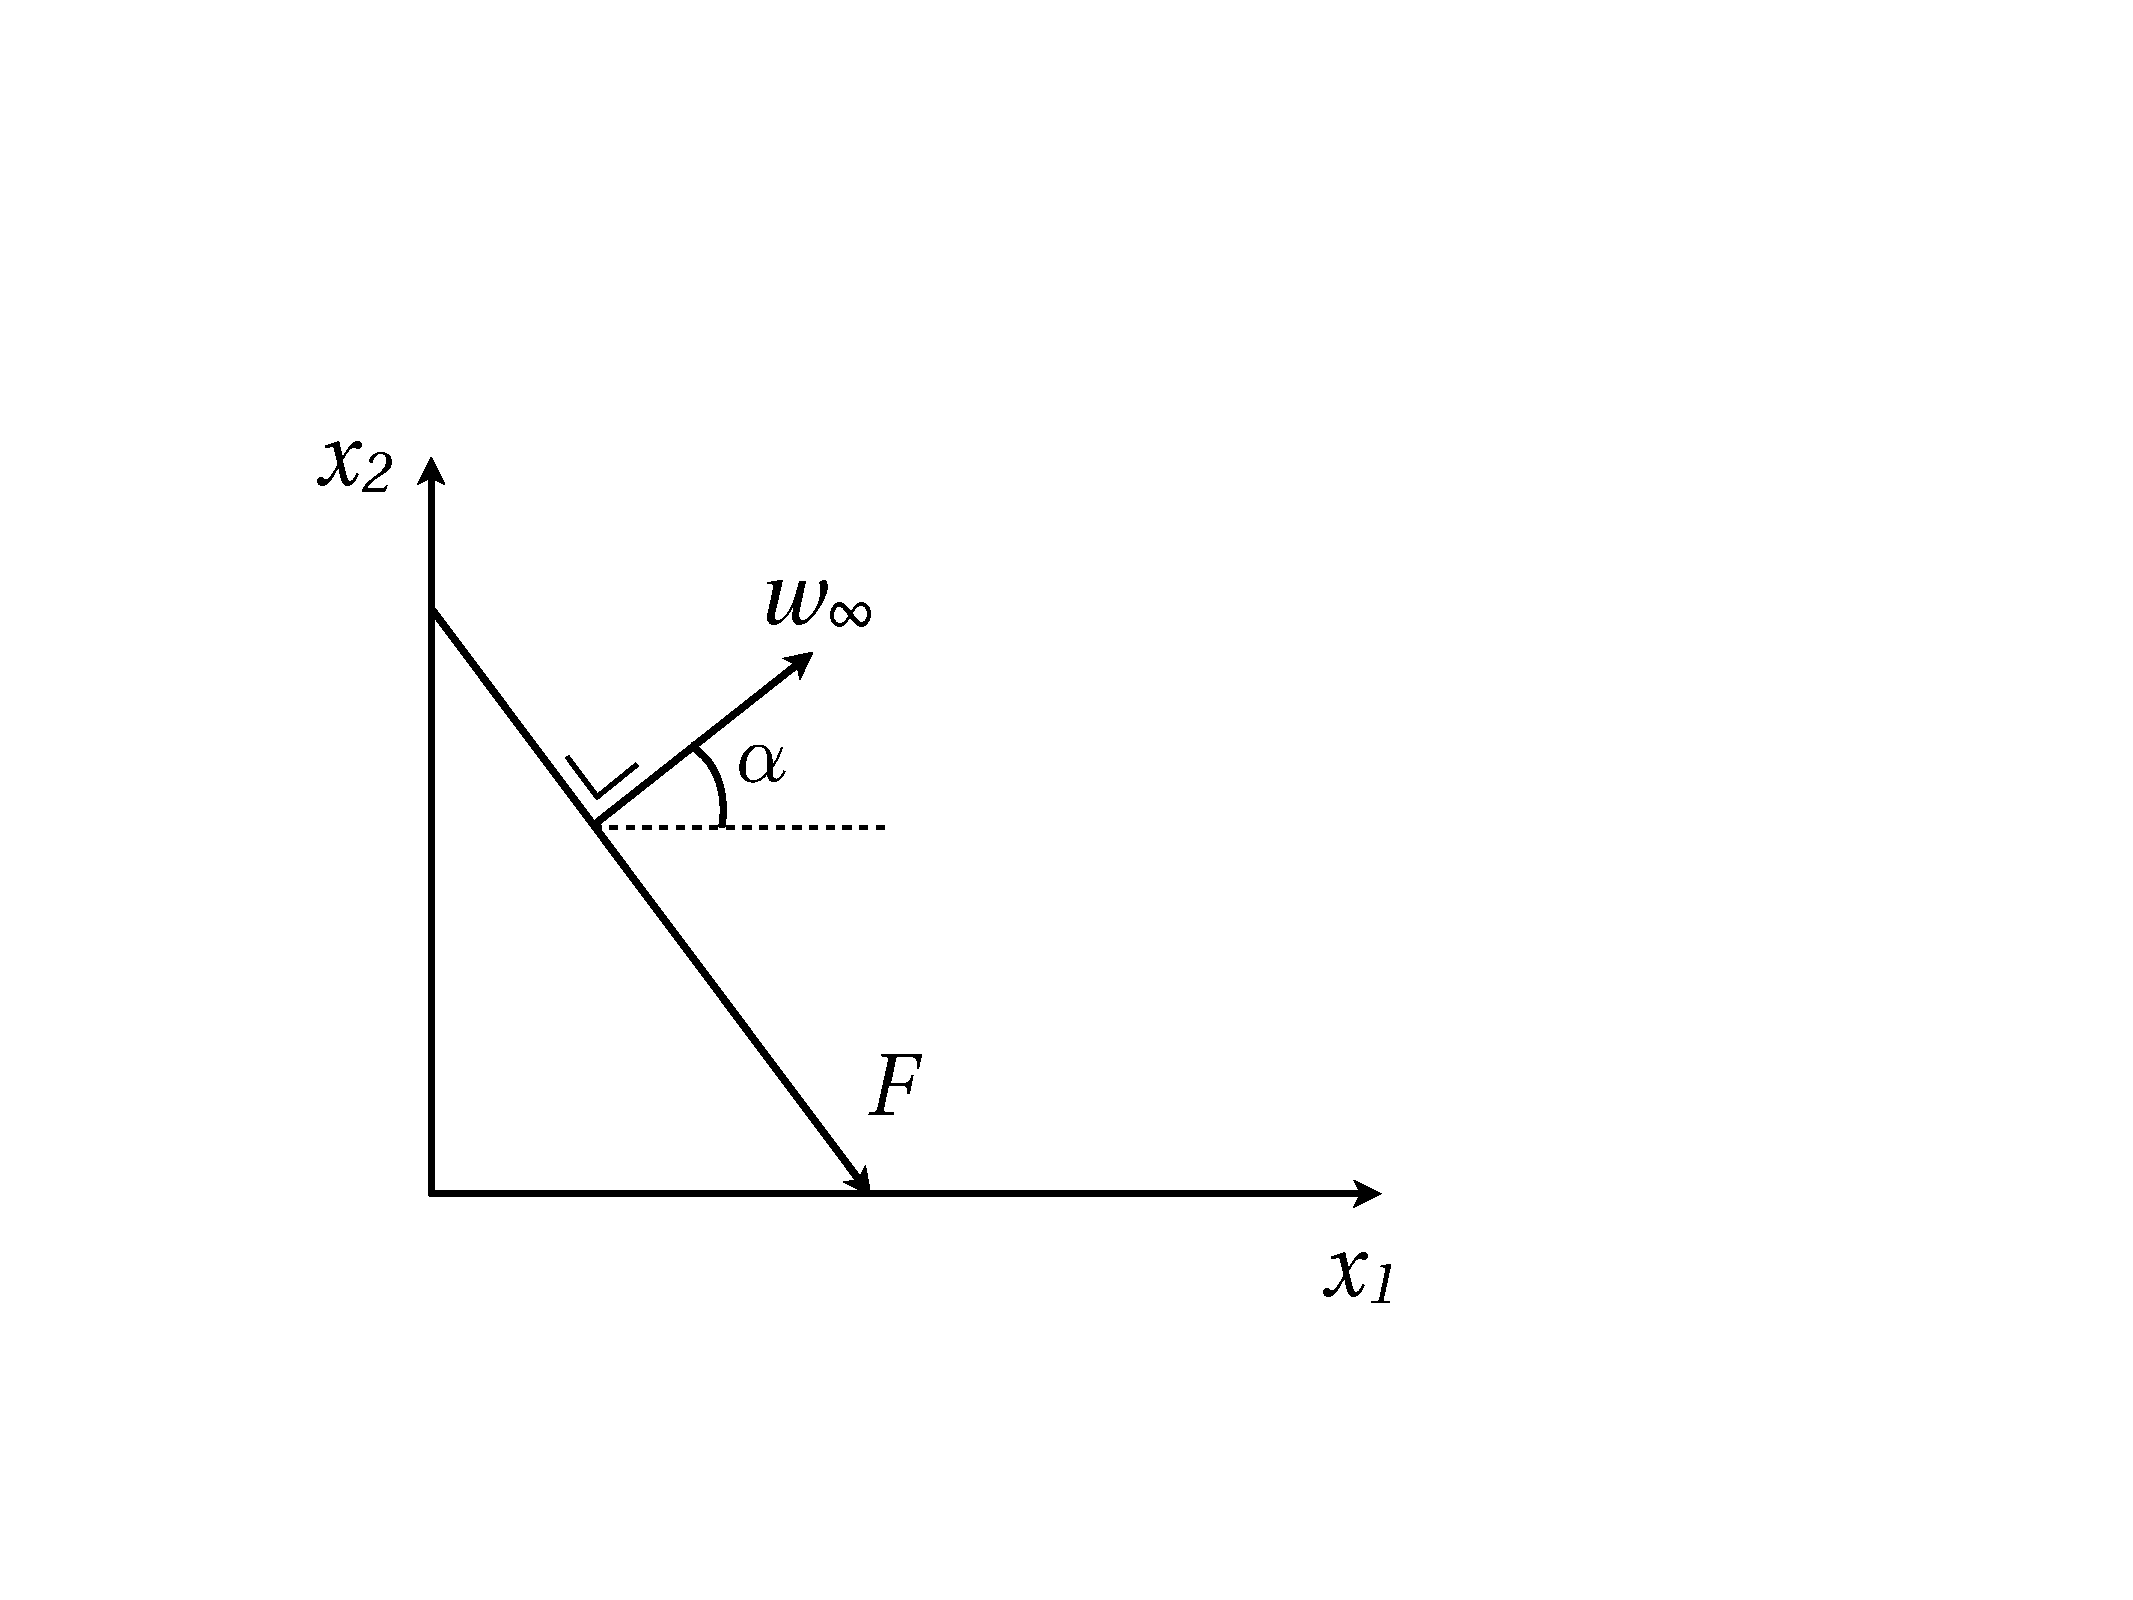
\includegraphics[scale=0.18]{ch3/8}	
		\captionof{figure}{}
		\end{wrapfigure}
	This is true independantly of the shape of the body. As first observation, we can see that if $u_\infty$ makes an agnle $\alpha$ with $x_1$ axis, the force is applied with an angle $\alpha - \pi /2$ meaning that it is $\perp u_\infty$. This means that there is no need of power to move a body in the velocity direction, no resistance. This is called \textbf{d'Alembert's paradox}. \\
	The second observation is that the magnitude $|F| = \rho u_\infty\Gamma$, where $\Gamma$ is the circulation. So we can create a perpendicular force (lifting force) by only generating a circulation, whatever the shape of the body. 
	
\section{Flow around a circular cylinder}
	\begin{wrapfigure}[8]{r}{5.7cm}
	\vspace{-5mm}	
	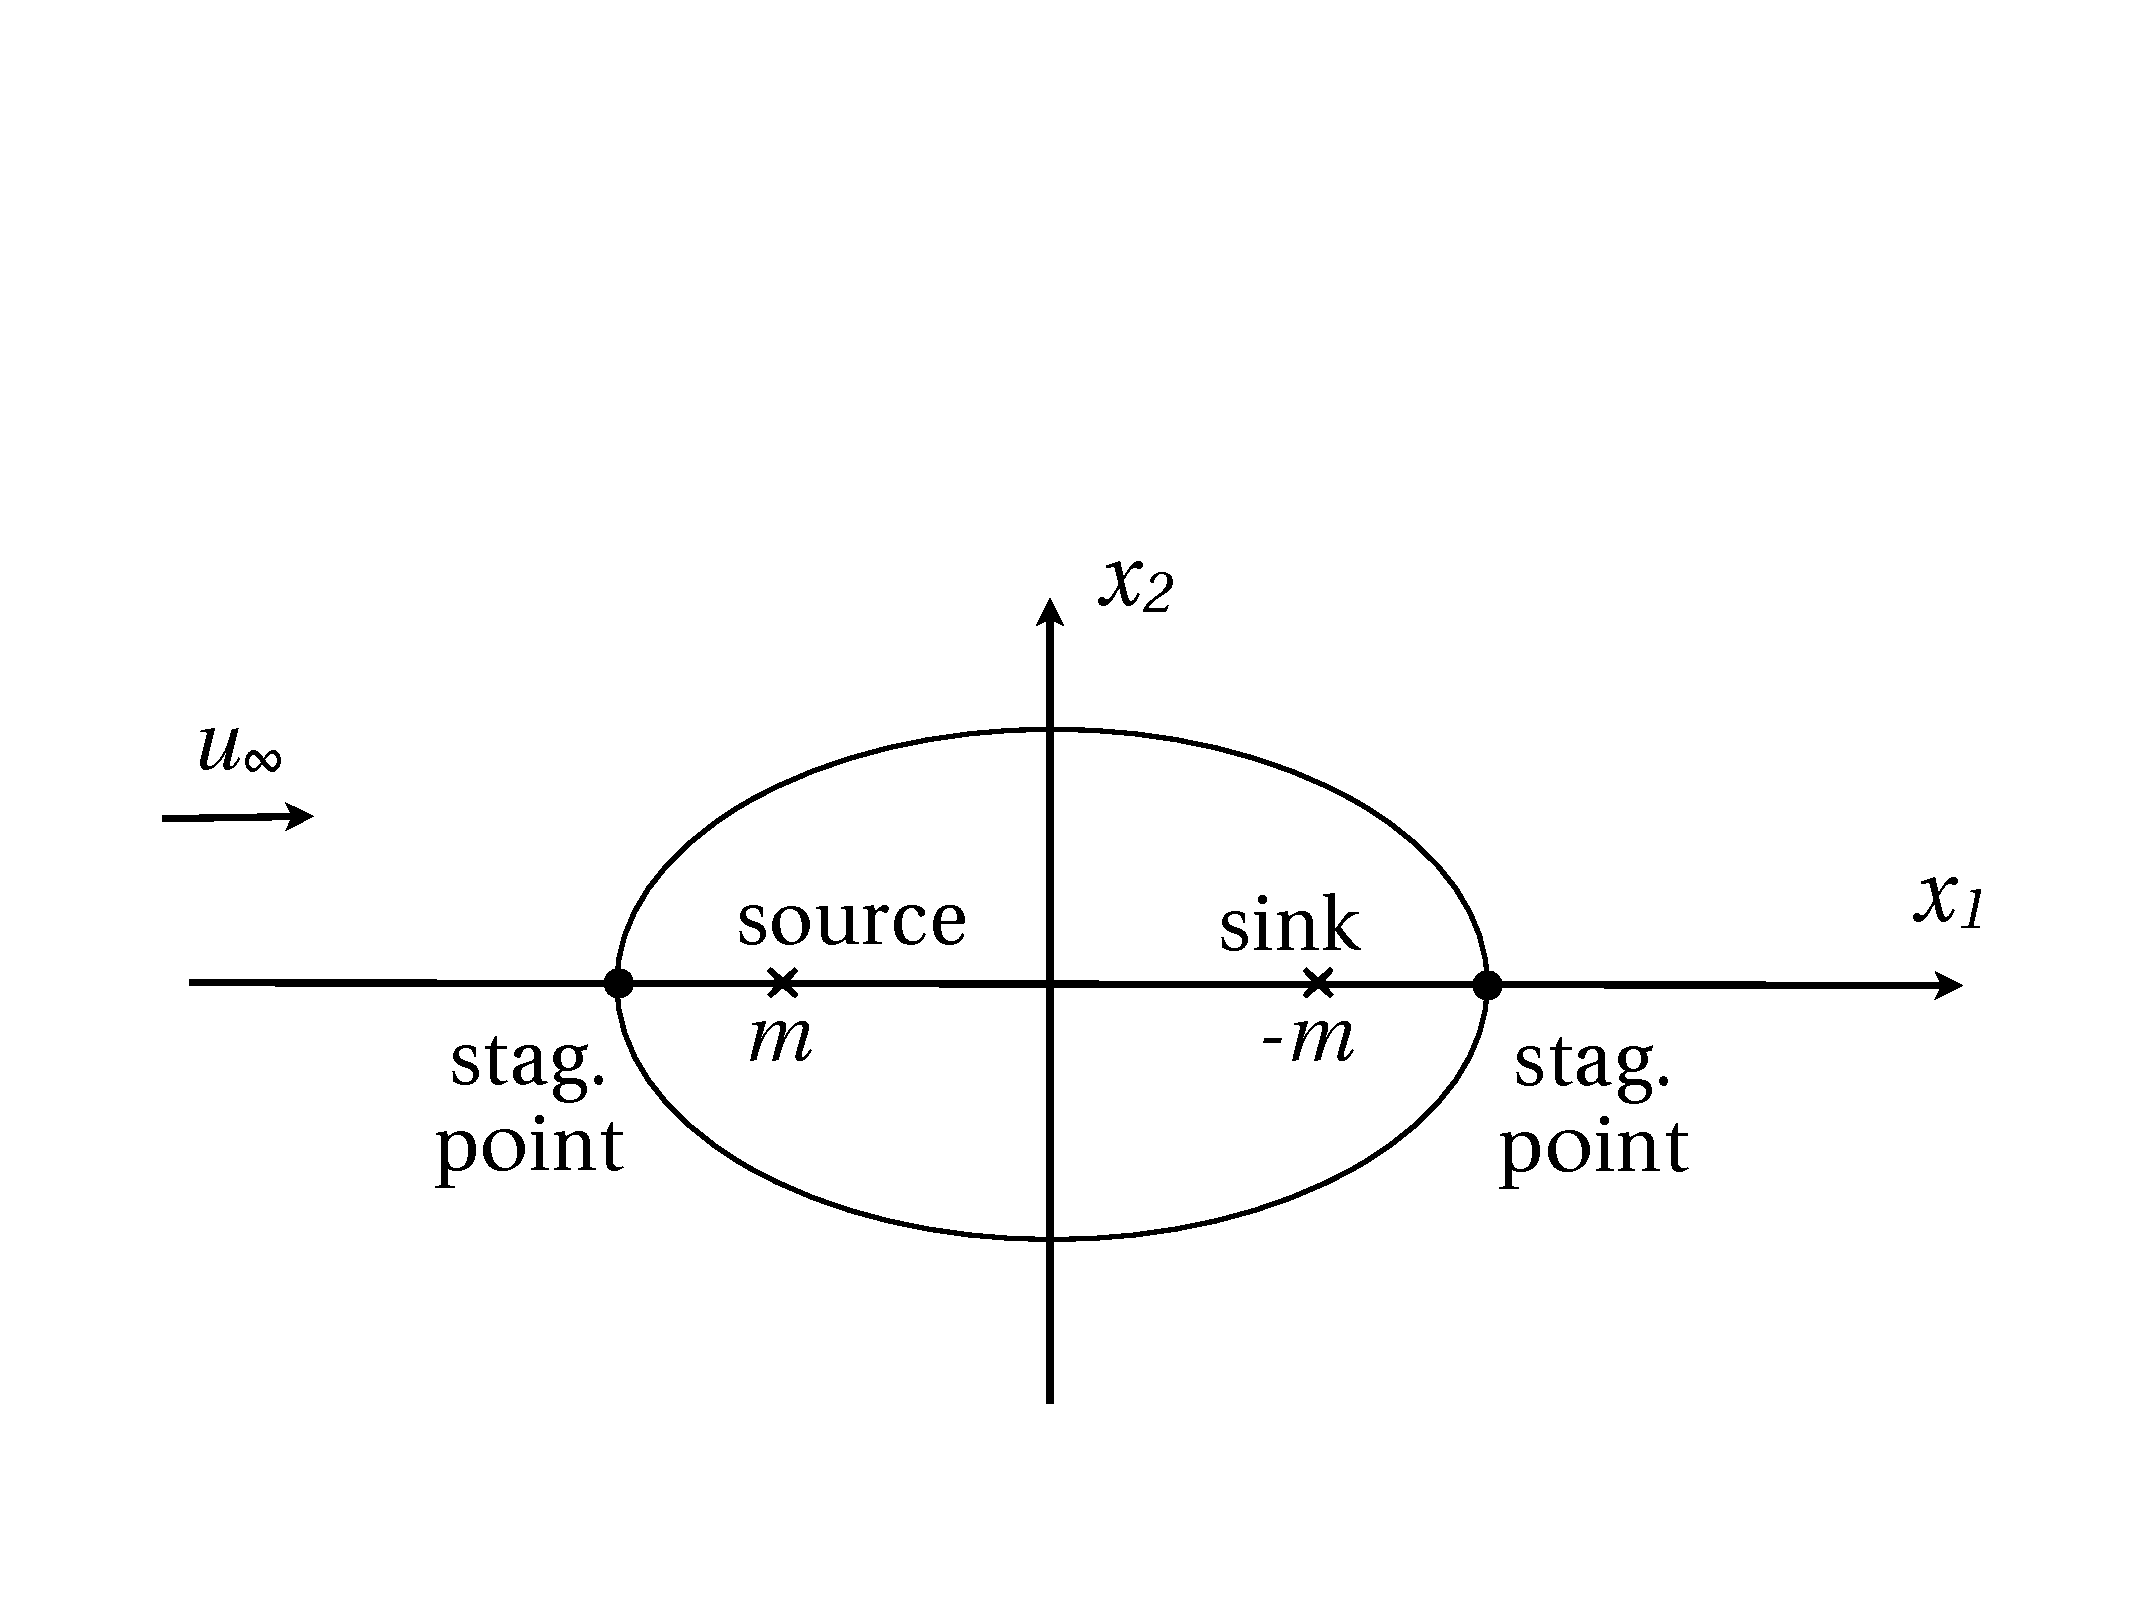
\includegraphics[scale=0.18]{ch3/9}	
	\captionof{figure}{}
	\label{fig:3.8}
	\end{wrapfigure}
	Knowing that it is possible to create complex shapes by composing sources and sinks and  that a closed streamline can be represented by a solid body (with singularities inside), the limiting case of a doublet flow superposed on a uniform flow can be considered, around a cylindre. We know that the flow generated by the source/sink is radial and the velocity is inversely proportional to the distance to the source/sink. There are 3 velocities to consider as a vector: $u_\infty \rightarrow$, $u_{source}\leftarrow$ and $u_{sink}\rightarrow$ with a magnitude varying with space. We are claiming that there is a point where the \textbf{velocity is null} and his symetric point, called the \textbf{stagnation point}. So there is a streamline going from one stagnation point to the other and symetrically in the other side of the real axis. This makes sense because there are two singularities inside the contour (not analytic), the flow goes from source to sink, wheras out of the contour, velocity is analytic. We will see how $u_\infty , 2a$ and $\dot{V}$ affect the shape of the body by having $\dot{V}/(u_\infty a)$ non dimensional that controls the shape. The limiting case is when $a \rightarrow 0, \dot{V} \rightarrow \infty$ and this becomes a doublet. Let's see what's hapening in this limiting case with the complex potential
	\begin{equation}
		\chi (z) = \chi _\infty(z) + \chi _{doublet}(z) = u_\infty z + \frac{\mu}{2\pi z}
		\label{eq:3.48}
	\end{equation}

	\begin{wrapfigure}[3]{l}{4cm}
	\vspace{-15mm}	
	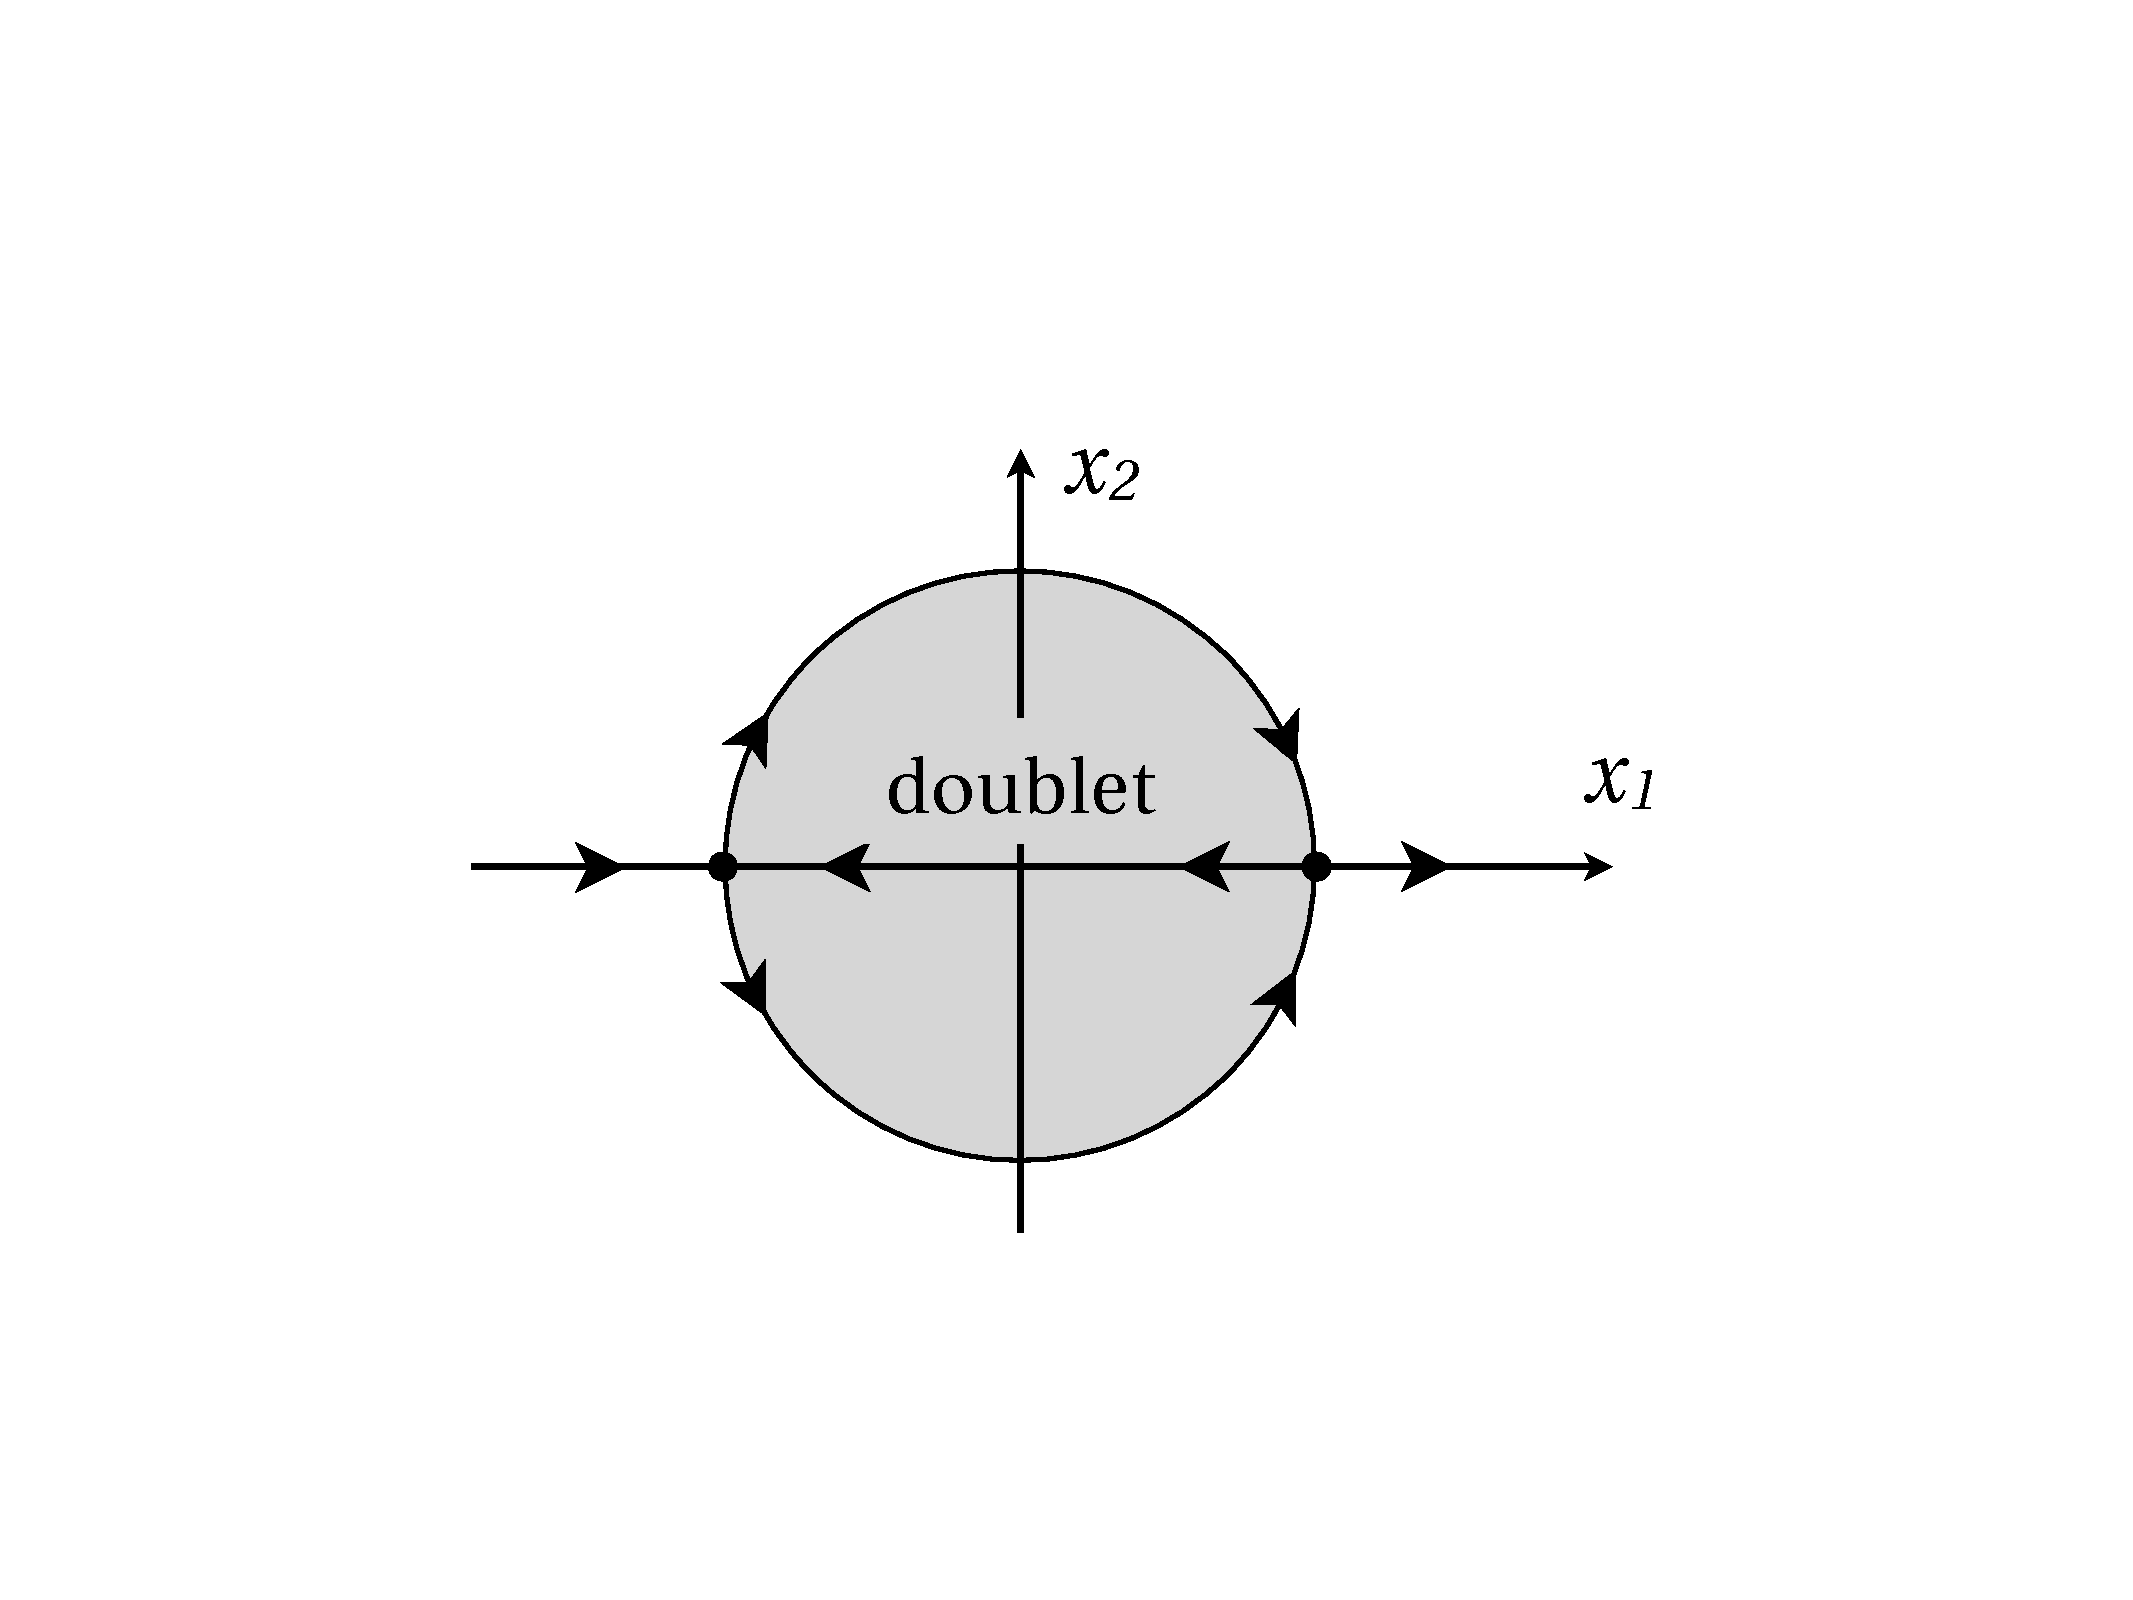
\includegraphics[scale=0.18]{ch3/10}	
	\captionof{figure}{}
	\label{fig:3.10}
	\end{wrapfigure}
	where the "+" sign is due to the orientation in $-x_1$ of the doublet and not in $x_1$, the doublet is facing the flow. The associated velocity and the stagnation point are 
	
	\begin{equation}
		w(z)  = u_\infty - \frac{\mu}{2\pi z^2}\qquad \Rightarrow \qquad w=0\quad \begin{aligned}
		&\Leftrightarrow  u_\infty - \frac{\mu}{2\pi z^2} = 0 \\
		&\Leftrightarrow  z = \pm\sqrt{\frac{\mu}{2\pi u_\infty}}=\pm a \\
		&\Leftrightarrow  \mu = 2\pi u_\infty a^2
		\end{aligned}
	\end{equation}
	 where $\pm a$ are the two positions of the stagnation points. We can replace in \eqref{eq:3.48} to obtain the equation of streamlines 
	\begin{equation}
		\chi = u_\infty \left( z+ \frac{a^2}{z} \right)\qquad \Rightarrow \psi = \operatorname{Im} (\chi) = u_\infty \left( x_2 - \frac{a^2x_2}{x_1^2+x_2^2}\right) = u_\infty x_2 \left( 1 - \frac{a^2}{x_1^2+x_2^2}\right) .
	\end{equation}
	We see that at the stagnation point $(x_2=0)$, $\psi (stag) = 0$. In fact there are two solution to this 
	\begin{equation}
		x_2 = 0 \qquad and \qquad 1 - \frac{a^2}{x_1^2+x_2^2} = 0  \Leftrightarrow x_1^2 +x_2^2 = a^2 \mbox{ (circle)}
	\end{equation}
	The streamlines are represented in \autoref{fig:3.10}\footnote{Don't forget that the flows goes from sink to source.}. We have composed the flow over a cylinder. In $w(z)$ there isn't a $1/z$ term so there isn't a $B_1$ for Laurent series, meaning that circulation $\Gamma = 0$, so there is no force. To explain this, let's analyse the pressure distribution.
	
	\subsubsection{Pressure distribution}
		The velocity over the circle is 
		\begin{equation}
		\begin{aligned}
			w(z) &= \uinf \left( 1-\frac{a^2}{z^2}\right) \qquad z = ae^{i\theta}\quad 0\leq \theta \leq 2\pi \\
			\Rightarrow \qquad w(\theta ) &= u_\infty \left( 1 - \frac{a^2}{a^2 \ e^{2i\theta}} \right)
 = u_\infty  e^{-i\theta} \left( e^{i\theta} - e^{-i\theta} \right) 
= 2  u_\infty  \sin \theta \,  e^{-i \left(\theta - \frac{\pi}{2}\right)}
		\end{aligned}
		\end{equation}
		This makes sense because if we consider a point of angle $\theta$, the velocity is tangential to the diameter with angle $\theta - \pi /2$ as it should. We also see that the magnitude is $u = 2  u_\infty  \sin \theta$, the velocity accelerates from stagnation point, reaches its maximum on $\theta = \pi /2$ and decelarate to 0 till the stagnation point. We can now get the pressure with Bernoulli, but first let's introduce a \textbf{non-dimensional pressure} for the special case of \textbf{inviscid potential flows}
		\begin{equation}
			C_p = \frac{p-p_\infty}{\rho \frac{\uinf ^2}{2}} \qquad \mbox{(denom : far field dynamic pressure)}.
		\end{equation}
		Bernouilli's equation is valid in the far field too, so replacing $p_t$ by its value we have
		\begin{equation}
			p = p _\infty + \rho\frac{\uinf ^2}{2}- \rho\frac{u^2}{2} \qquad \Rightarrow \frac{p-p_\infty}{\rho \frac{\uinf ^2}{2}} = 1- \left(\frac{u}{\uinf}\right) ^2 = 1 - 4\sin ^2 \theta
		\end{equation}
		where the final result is obtained by considering $u$ for a circular cylinder. We have a single formula for all cylindres and all velocities (independant). If we take two opposite value of $\theta$, we have the same pressure, also for $\pi - \theta$ ($\sin$). It is symetric to $x_1$ and $x_2$ axis, the four forces cancelling each other (normal and tangential components) making sense with d'Alembert's paradox. 
		
		\begin{wrapfigure}[9]{l}{6cm}
	\vspace{-5mm}	
	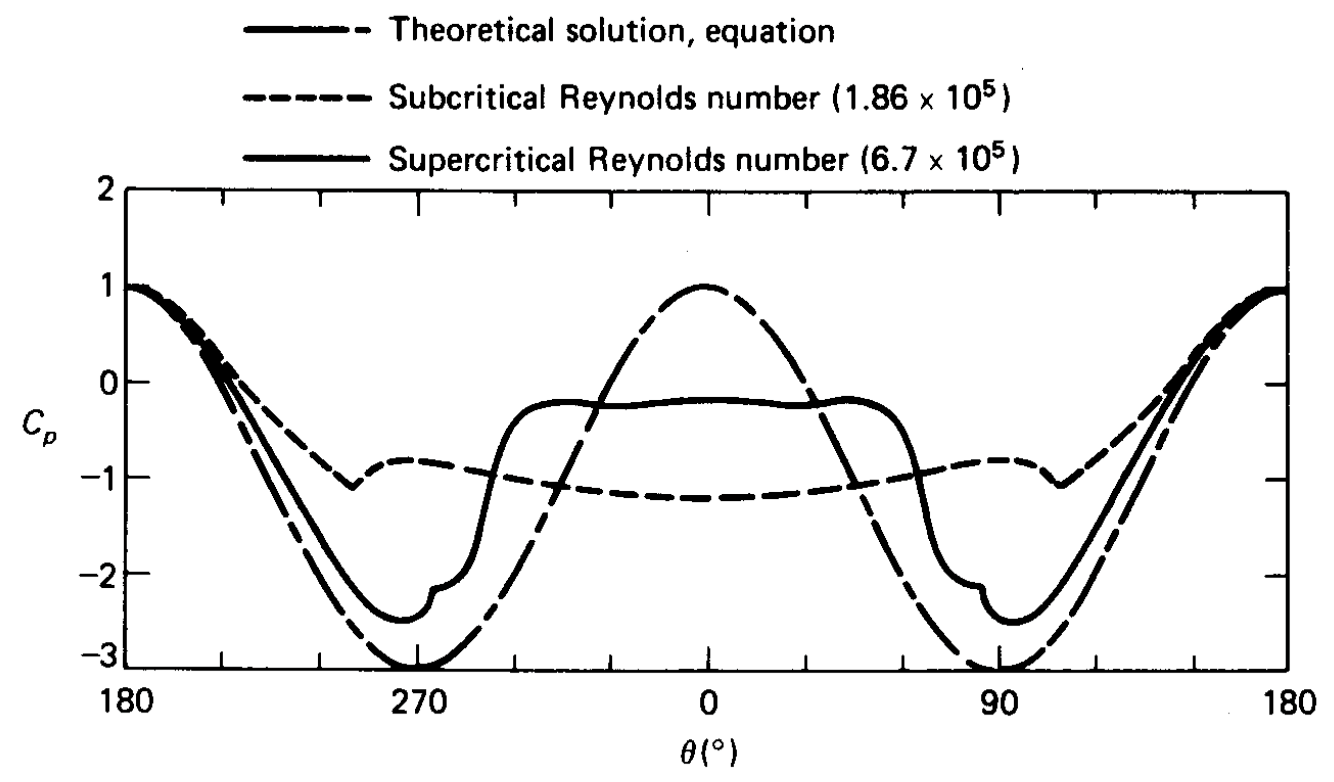
\includegraphics[scale=0.25]{ch3/12}	
	\captionof{figure}{}
	\end{wrapfigure}
	The real case only match with this at the instant directly after start of the flows. After a couple of time, there is creation of vorticies at the back that makes the stramlines deviate and the velocity distribution don't correspond to a $\sin$. This effect is large for low $Re$ numbers but tend to disappear for high $Re$ number, making the flow turbulent. For turbulent flows, the separation/deviation appear more on the back ($\approx -\pi/2 < \theta < \pi /2$). This method is used on golf balls by designing dimpels. 
		
	\subsubsection{Adding a concentrated vortex}
		
	\begin{wrapfigure}[5]{r}{6cm}
	\vspace{-5mm}	
	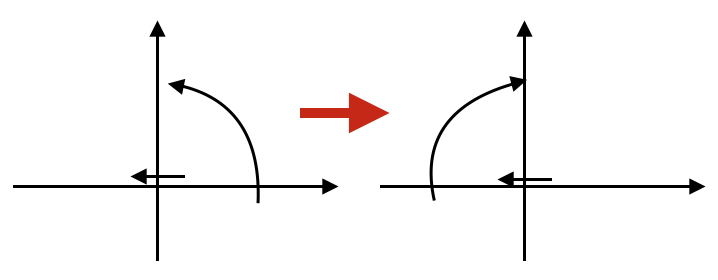
\includegraphics[scale=0.45]{ch3/11}	
	\captionof{figure}{}
	\label{fig:3.11}
	\end{wrapfigure}
	Now the question is to determine if the solution (the flow) we found is the only solution. We have already seen that we have circular streamlines for a concentrated vortex. Let's supperimpose to this flow, the flow due to a concentrated vortex (doublet + uniform + vortex). Normally a vortex is represented as left in \autoref{fig:3.11} but corresponds to the case of a force with angle $\alpha -\pi /2$ in \autoref{fig:3.8}. We will consider a lifting force so the clockwise orientation for the vortex and an angle $\alpha + \pi /2$. The new complex potential becomes 
	\begin{equation}
		\chi = \uinf \left( z+\frac{a^2}{z^2} \right) + \chi _\Gamma = \uinf \left( z+\frac{a^2}{z^2} \right) + \frac{i\Gamma}{2\pi}\log z .
	\end{equation}
	If we compute now the streamlines and check their expression on the circle $x_1^2 + x_2^2=a^2$
	\begin{equation}
	\begin{aligned}
	\psi &= \operatorname{Im}(\chi) = u_\infty  x_2 \left( 1 - \frac{a^2}{x_1^2 + x_2^2} \right)+ \operatorname{Im} \left[ \frac{i \Gamma}{2 \pi} \left( \frac{\ln (x_1^2 + x_2^2) + i\theta }{2} \right) \right]\\
 &=u_\infty  x_2 \left( 1 - \frac{a^2}{x_1^2 + x_2^2} \right)+ \frac{\Gamma}{2 \pi}\ln \left(\sqrt{x_1^2 + x_2^2}\right)\\
 \Rightarrow \qquad \psi &_{circ} = 0 + \frac{\Gamma}{2\pi}\ln a = cst 
	\end{aligned}
	\end{equation}
	We see that there isn't only one solution admitting the circle as $\psi$, there are an infinity of solutions dependant of $\Gamma$. Now what will be the value of $\Gamma$? For a circular cylinder there is no reason to have a circulation as the previous discussion demonstrated, unless we rotate the cylindre in the direction of the potential due to the viscous layer that induces circulation (creates lift). Let's check the stagnation points on the circle $z = ae^{i\theta}$
	\begin{equation}
	\begin{aligned}
		w &= \uinf \left( 1-\frac{a^2}{a^2e^{i2\theta}}\right)+\frac{i\Gamma}{2\pi ae^{i\theta}} = \uinf 2ie^{-i\theta}\sin \theta + \frac{i\Gamma}{2\pi ae^{i\theta}}\\
		 &= e^{-i(\theta -\pi /2)}\left( 2\uinf \sin \theta + \frac{\Gamma}{2\pi a} \right) \quad \Rightarrow w = 0 \Leftrightarrow \sin \theta = -\frac{\Gamma }{4\pi a \uinf}
	\end{aligned}
	\end{equation}
	We see that the previous position is not remaining, the two point are displaced to the lower part of the cylindre but the line joining them remains parallel to the flow. If we reach a $\sin > 1$, the unique stagnation point is outside the circle. \\
	
	For the pressure distribution we have 
	\begin{equation}
		C_p = 1-\left( \frac{u}{\uinf} \right)^2 = 1 - \left(2\sin \theta + \frac{\Gamma}{2\pi a\uinf} \right) ^2.
	\end{equation}
	Actually for the velocity, we have a larger velocity at the top $\pi/2$ and a lower velocity at $-\pi /2$ because of the positive and then negative contribution of the concentrated vortex. This implies that the pressure is higher below than at the top that creates a lift force. What should be the rotational velocity? The correspondance between angular velocity and the one induced by the vortex is
	\begin{equation}
		wa = \frac{\Gamma}{2\pi a} \qquad \Leftrightarrow	\qquad w = \frac{\Gamma}{2\pi a^2}.
	\end{equation}
	\ \\ 
	\begin{wrapfigure}[7]{l}{4.8cm}
	\vspace{-15mm}	
	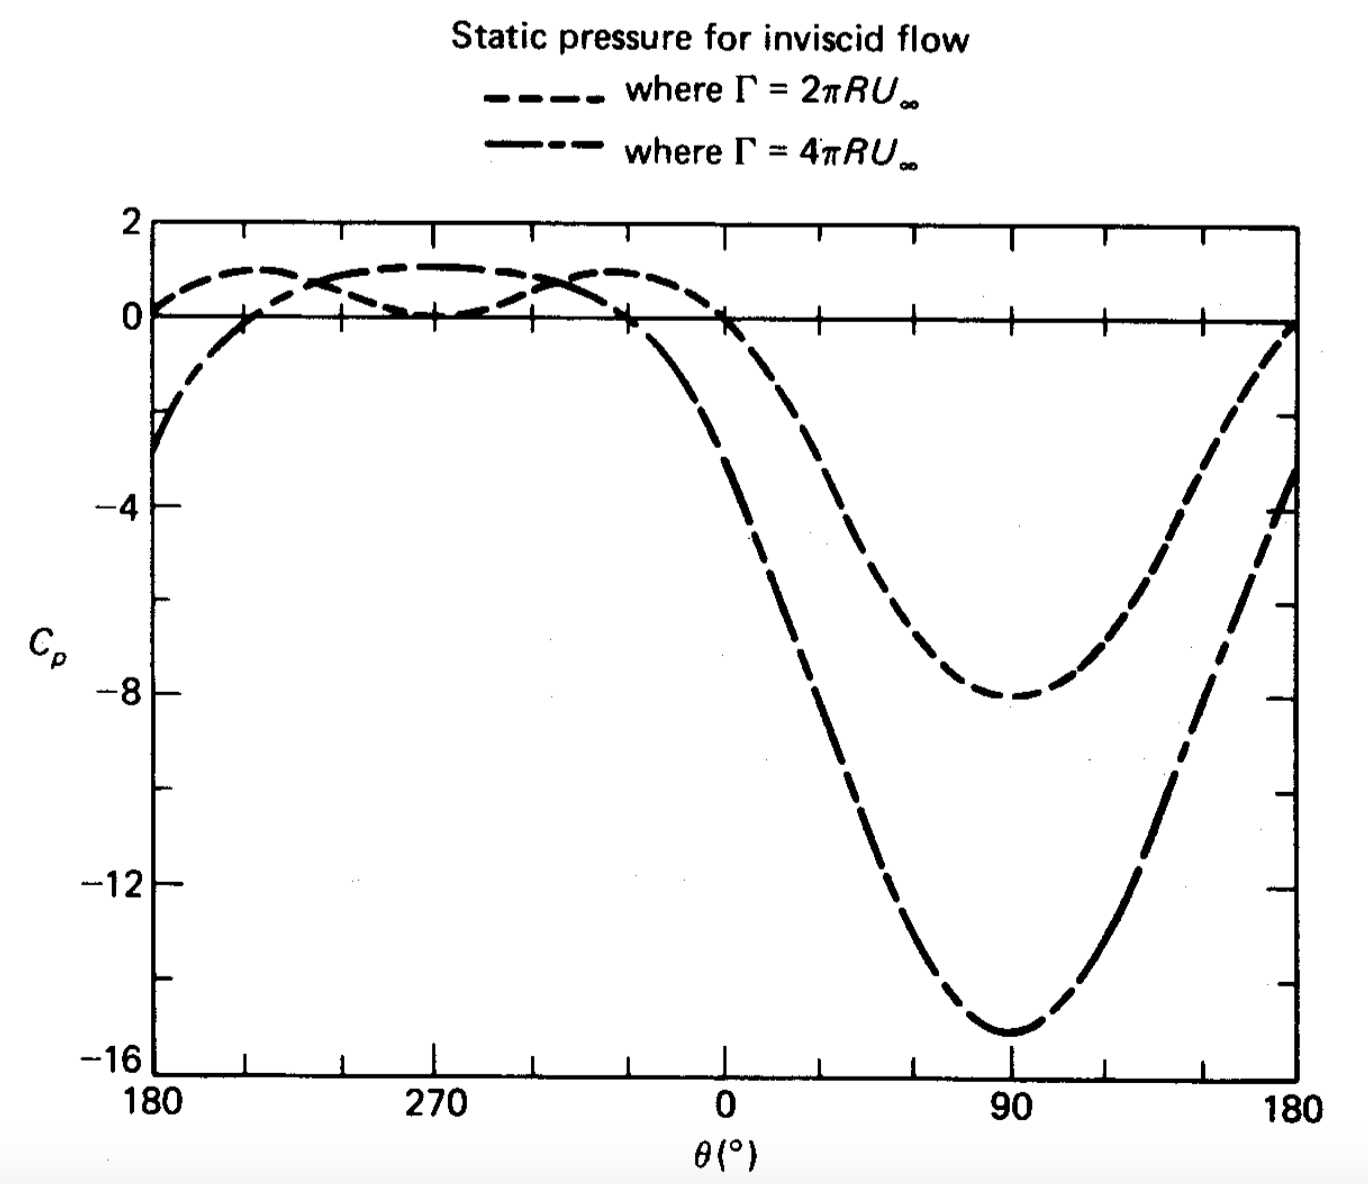
\includegraphics[scale=0.2]{ch3/13}	
	\captionof{figure}{}
	\label{fig:3.13}
	\end{wrapfigure}
	This is the theoretical result, in practice we have to rotate twice that velocity. \autoref{fig:3.13} confirms our conclusion. Notice that most of the force are not caused by an overpressure on the lower part but by an underpressure on the upper part, leading to consider the air over a wing for example as sucking the wing upper. 